% vim: set tw=78 tabstop=4 shiftwidth=4 aw ai:

\chapter{Deploying Peer-to-Peer Network Infrastructures through
Virtualization}
\label{chapter:virt-infra}

Due to the large number of research and development efforts for designing and
implementing new applications, hardware components, network protocols,
services, the existence of suitable test environments is essential.
Functionality testing, performance evaluation, user experience evaluation have
to be undertaken to ensure quality and compliance of future products.

Test environments for software testing are nowadays an integral part of the
software development cycle. Specialized systems or setups allow developers or
quality engineers to subject their applications to various conditions in order
to grade their functionality, standard compliance, performance etc. The rapid
advance of virtualization technologies and cloud computing have enabled rapid
deployment of testing environments and quick decommission when they are no
longer required.

With respect to network protocol and applications, two kinds of environments
are generally used for testing, measurements, evaluation and analysis: lab
setups and real world experiments. Lab setups or experimental setups are
custom setups for protocol evaluation; the experimenter has full control of
the environment. This is typically the case for functionality testing or
experiments in which the experimenter needs full control of the process. The
experimenter may use a lab-based infrastructure, a cluster/cloud based one, or
one provided by the community, such as
PlanetLab\footnote{\url{http://www.planet-lab.org/}}. Rias~\cite{rias} is an
example of an overlay topology created on top of a PlanetLab infrastructure.

Large scale scenarios are deployed in the Internet and allow limited control
for the experimenter. Large BitTorrent experiments such as those employed by
Pouwelse~et~al.~\cite{measurement-study} use existing infrastructures and
participants. The purpose of large scale scenarios is to collect statistical
information from real world sessions and subject it to dissemination. The
experimenter has little or no control over the setup; the purpose is to
analyze a protocol, class of protocols, applications or participants in a real
world environment. Most challenges revolve around the ability to collect
information, upset by peer connectivity and relevance.

Our work presents an custom Peer-to-Peer infrastructure to be used mostly for
lab setups; it can be integrated in the larger ``Internet cloud'' as part of a
larger swarm. The main goal is to ensure an easily deployable and customizable
platform for Peer-to-Peer experiments with the possibility of completely
defining peer behavior and network characteristics. The infrastructure has
been successfully employed in several experiments regarding BitTorrent
implementations~\cite{bt-pef} and provided important results regarding peer and overall
swarm performance.

The aim is to provide an automated, extensible, scalable, realistic, easy to
use and deploy, efficient and general purpose infrastructure for Peer-to-Peer
networks. The infrastructure uses virtualization~\cite{p2p-va} as the means for
providing a large number of Peer-to-Peer ``nodes'' and an will employ a
plethora of tools required to create a realistic environment such as creating
bandwidth limitation, selecting node characteristics and ensuring automation.
The infrastructure forms the basis for deploying medium-scale experiments that
provide valuable insight in the behavior of the Peer-to-Peer protocols,
through analysis of protocol parameters.

\section{Virtualization. OpenVZ}
\label{sec:virt-infra:openvz}

An important ``buzzword'' in the last decade, virtualization technology has
broken ground from its theoretical base in the late 70s to a diversity of
full-fledged implementations nowadays. With the continuous increasing capacity
of HDD space, memory and CPU power (mostly in number of cores), virtualization
solutions provide the best way for proper allocation of resources. New
features such as hardware-assisted virtualization, I/O improvements, live
migration have ignited the demand for efficient virtualization solutions that
consolidate current and future hardware resources.

Cloud computing, an already established technology in modern Internet, makes
heavy use of virtualization in order to satisfy user demands while cutting
hardware and software infrastructure costs. Major players such as Amazon,
Microsoft and Rackspace deploy important virtualization solutions such as Xen,
KVM and Hyper-V.

Generally speaking, virtualization refers to mechanisms for providing a
similar interface on top of an existing entity. That entity may be a program
(\textit{software virtualization}, e.g. {Java Virtual Machine}),
a concept (e.g. \textit{memory virtualization}, or a computer system
(\textit{hardware virtualization}). We will focus on hardware virtualization,
as it this the most common form for use of the word \textit{virtualization}
and as it forms the basis of our work.

Although difficult to give out a proper description of virtualization, Dittner~et~al.~\cite{best-damn-virt} give the following definition: \textit{A framework
or methodology of dividing the resources of a computer hardware into multiple
execution environments, by applying one or more concepts or technologies such
as hardware and software partitioning, time-sharing, partial or complete
machine simulation, emulation, quality of service, and many others}.

Virtualization solutions allow instances of operating systems to run on top of
another operating system. The base operating system offers an interface very
similar to the hardware it runs on. The base OS or application that offers the
hardware-like interface is called a \textbf{virtual machine monitor} (VMM) or
\textbf{hypervisor}. Depending on the virtualization solution, the hypervisor
may be an operating systems running directly on top of the bare hardware (e.g.
Xen, Hyper-V) or an application running within an operating system (e.g.
VMware Workstation, OpenVZ).
Figure~\ref{fig:virt-infra:hardware-virtualization} depicts the general
architecture of a virtualization solution.

\begin{figure}
  \centering
  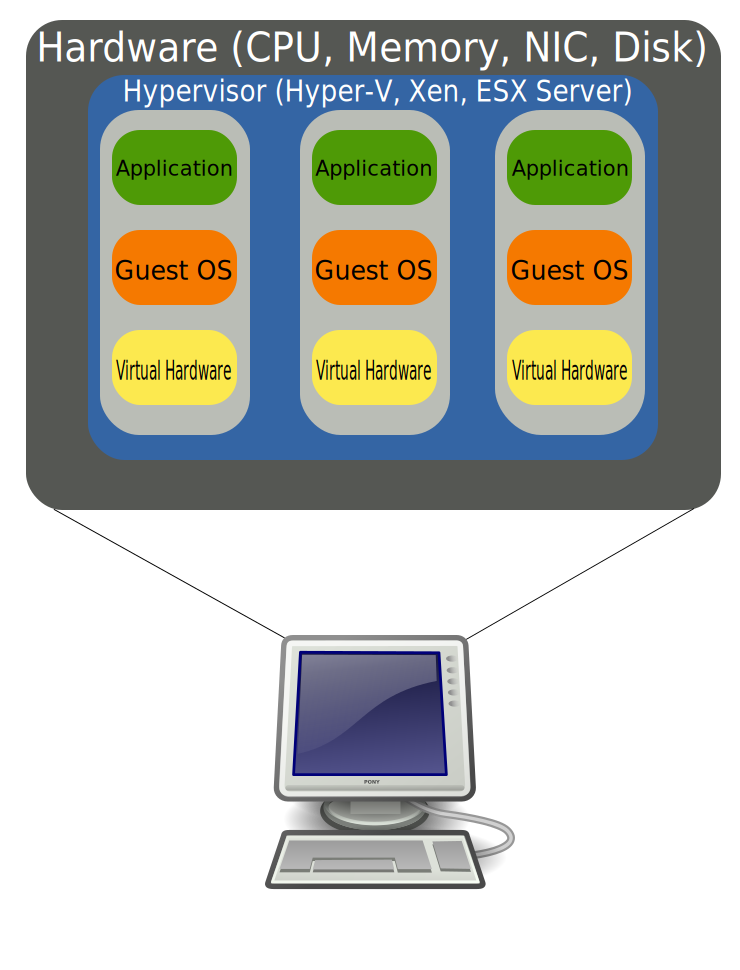
\includegraphics[width=0.5\textwidth]{src/img/virt-infra/hardware-virtualization}
  \caption{Hardware Virtualization}
  \label{fig:virt-infra:hardware-virtualization}
\end{figure}

The existence of the VMM, just as the kernel mode/user mode separation, is
possible in modern processors because of the existence of a supervisor mode
allowing for privileged instructions. Modern virtualization solution will try
to execute as much of the virtual machine's instructions as possible on native
hardware. Recent updates to x86 architecture, such as Intel-VT and AMD-V have
enabled proper hardware assisted virtualization allowing high performance.
Performance of virtual machines had been considered by
Bratanov~et~al~\cite{virt-analysis}; they created a testing and benchmarking
environment and considered aspects such as overhead, precision and scope.

\subsection{Benefits of Virtualization}

Virtualization solutions have made their way in day-to-day uses as they
provide important benefits, especially regarding costs. A specific hardware
system may be able to run different instances of operating systems, while, in
the absence of virtualization, more systems would be required.

Three important benefits have been identified~\cite{best-damn-virt} for
virtualization:

\begin{itemize}
  \item consolidation;
  \item reliability;
  \item security.
\end{itemize}

\textbf{Consolidation}, a particularly important aspect in the business world,
allows the ``unification'' of resources on top of a few physical platforms. The
ever increasing CPU power, I/O speed and memory capacity may now be used to
provide sufficient resources for multiple virtualized operating systems.
Modern data centers must be plugged even when nothing is really running,
resulting in infrastructure waste. The use of virtualization solutions and
migration techniques allows the unification of multiple virtual servers on
shared hardware.

Consolidation also allows old applications to run on legacy systems. Migrating
an application to another server results in compatibility issues. With the
help of virtualization, applications will run on the same virtualized platform
that may be migrated to a different physical platform.

Not least, development and test environments may be easily deployed and
decommissioned. As development and test environments do not imply perennial
use, such as production environments, one may allocate several virtual
machines, consolidate workload on a few physical servers and then scrap or
disable those virtual machines and regain virtual servers. This allows both
flexibility of the development and testing environment and infrastructure
savings.

Virtualization solutions provide \textbf{reliability} through isolation. A
failure on a given virtual machine will not affect another virtual machine.
The ``partitioning'' employed by a virtualization solution means that each
virtual machine is running on a dedicated specialized simulated hardware. The
isolation and partitioning allow dynamic allocation of new systems whenever
required without the need to acquire additional hardware.

Just as typical data centers provide failover servers to maintain system
availability, virtualization may be used to provide software based
provisioning of additional systems when required. In a typical cluster, a
failover node has to be active and online. Using virtualization, failover
nodes may be collocated on fewer physical hosts reducing hardware investments.

Isolation provided by virtualization technology is a key feature for ensuring
security of virtual machines. If a given virtual machine faults or has been
compromised, it does not affect other systems and, in need, it may be rapidly
disabled. This would be very difficult to achieve on a physical
infrastructure.

Each virtual machine possesses its own security settings and configuration
directives. This means that each virtual machine may be administered
separately: an administrative (root) account on a given virtual machine will
have no impact on another machine. Each administrator would configure its own
virtual machine by need, leaving the physical platform to be administered by
the solution provider. Virtualization thus allows delegation and isolation of
full administrative rights on the same hardware system.

\subsection{Types of Virtualization Solutions}

As mentioned before, virtualization, in the general sense, may refer to
hardware/server virtualization, software/application virtualization,
storage/memory/network virtualization.

As this work uses a particular type of server/hardware virtualization (namely
operating system level virtualization), focus will be given to this. The most
dominant form of virtualization, server virtualization, allows the coexistence
of multiple operating systems on the same physical platform. A Virtual Machine
Monitor (VMM) or hypervisor provides a hardware like interface for virtual
machines and the operating systems running within those.

Although various classifications exist, we will present the types described by
Dittner~et~al.~\cite{best-damn-virt}:

\begin{itemize}
  \item full virtualization;
  \item paravirtualization;
  \item native virtualization;
  \item operating system virtualization.
\end{itemize}

\textbf{Full virtualization} is a virtualization technique that provides
complete simulation of the underlying hardware. The result is a system in
which all software capable of execution on the raw hardware can be run in the
virtual machine. Full virtualization has the widest range of support in guest
operating systems. Due to the specifics of the x86 architecture, full
virtualization may not be implemented in its pure form. Examples of
full virtualization solutions are host-based virtualization solutions such as
VMware Workstation, Virtual Box, Microsoft Virtual PC.

\textbf{Paravirtualization} is a virtualization technique that provides
partial simulation of the underlying hardware. Most but not all of the
hardware features are simulated. The key feature is address space
virtualization, granting each virtual machine its own unique address space.
However, without proper hardware support, operating systems running in
paravirtualized virtual machines have to be modified in order to run, which
may pose problems to the solution provider. Example of such solutions are Xen,
Microsoft Hyper-V, VMware ESX(i), Parallels Workstation.

\textbf{Native virtualization} is the newest to the x86 group of
virtualization technologies. Often referred to as hybrid virtualization, this
type is a combination of full virtualization or paravirtualization and
I/O acceleration techniques. Similar to full virtualization, guest
operating systems can be installed without modification. It takes advantage of
the latest CPU technology fo x86, Intel VT and AMD-V. Linux
KVM\footnote{\url{http://www.linux-kvm.org/}} is the most
well known implementation of native virtualization with VMware Workstation,
Xen and Microsoft Hyper-V enabling it in recent versions.

\textbf{Operating system-level virtualization} is a virtualization technique
where the operating system kernel allows multiple isolated (jailed) user-space
instances. Virtual machines are commonly called containers, virtual
environments (VEs) or virtual private servers (VPS). OS-level virtualization
allows all processes to run on top of the basic operating system kernel thus
enabling minimal overhead. While in normal virtualization solutions, a request
would pass through the virtual machine kernel and then, if required, through
the hypervisor, an OS-level virtualization solution required passage through
the base kernel. Example solutions include OpenVZ, LXC, BSD jails, Linux
V-Server. A graphical depiction of OS-level virtualization solutions is
presented in Figure~\ref{fig:virt-infra:os-level-virtualization}.

\begin{figure}
  \centering
  \includegraphics[width=0.7\textwidth]{src/img/virt-infra/os-level-virtualization}
  \caption{Operating System-Level Virtualization}
  \label{fig:virt-infra:os-level-virtualization}
\end{figure}

Due to its low overhead, OS-level virtualization is the preferred form of
virtualization for virtual private servers and virtual hosting. Its good
isolation, low overhead and efficiency allows the rapid creation and
deployment of a large number of containers. Its main disadvantages are the
lack of flexibility in running different kinds of operating systems (only an
operating system that may use the base kernel can be run) and the fact that a
kernel error is common to all containers and base OS.

The advantages of OS-level virtualization have boosted it as the number one
solution for creating the P2P network infrastructure described in this work.
With low overhead and easy deployment, OS-level virtualization allows the
creation of a high number of virtual machines and required resources. The
infrastructure has been deployed and put to use and results are
excellent~\cite{p2p-va};
while some issues still persist (such as the inability to use traffic shaping
tools within a containers) the benefits of using this technology outweigh the
disadvantages. A case study of the scalability of OS-virtualization solutions
for P2P environments has been presented by
Bardac~et~al.~\cite{p2p-virt-scaling}.

\subsection{OpenVZ}

As OS-level virtualization had proven to be the way to go for building up a
Peer-to-Peer infrastructure, we had to chose between existing solutions such
as OpenVZ, LXC, V-Server. As we have good experience with Linux, the solution
had to be a Linux-based solution. We had to chose between OpenVZ, LXC,
V-Server. Though LXC currently possesses the advantage of being active in the
mainline kernel, it was still in its infancy in the time we started building
the infrastructure. Apart from that, documentation is quite scarce. Between
OpenVZ and V-Server, we chose OpenVZ due to its high quality documentation
and peer recommendation and experience.

Just as other OS-level virtualization solutions, OpenVZ is a series of patches
to the Linux kernel that enhances process and resource isolation among
containers. Major Linux distributions typically ship an OpenVZ able kernel that
is easily installable. A series of user space tools allow installation and
configuration of virtual machines. Typically, most commands and keywords start
with the \texttt{vz} prefix.

OpenVZ is an open-source project provided by Parallels Inc. with the help of
an online community. Parallels provides a commercial product, Virtuozzo, as an
extended version of the OpenVZ project.

OpenVZ uses specific nomenclature and identifiers for physical platforms and
containers. The physical platform is typically called the \textbf{hardware
node}, and is referred through \textbf{HN}. As it is the container manager it
is also referred as \textbf{CT0} or \textbf{VE0}. Virtual machines are
typically called \textbf{containers} (\textbf{CTs}) or \textbf{virtual
environments} (\textbf{VEs}) (prefered term is container). Each container is
identified by a number, called \textbf{VEID} or \textbf{CTID}
(\textbf{container identifier}). CTID 0 is reserved for the hardware node.

User space tools (such as \texttt{vzctl}) are used for creating and
configuring OpenVZ containers. From a simplistic point of view, a container is
a Linux filesystem structure. The creation of a container requires creating a
complete Linux filesystem and then creating an OpenVZ specific configuration
file. The Linux filesystem is typically distributed in tarballs also called
OpenVZ templates. A template is uncompressed and deployed as a container.

For each OpenVZ container a user may configure:

\begin{itemize}
  \item hostname;
  \item network interfaces;
  \item mount point;
  \item quotas;
  \item modules;
  \item resource limits.
\end{itemize}

The ability to limit resources is one of the most important features for
OpenVZ with respect to building a testing environments. OpenVZ uses user
beancounters (UBCs) dubbed as resource management feature. The interface is
accessible in OpenVZ containers as the \texttt{/proc/user\_beancounters} entry,
soon to be changed to the \texttt{/proc/bc/} folder. The resource management
interface of OpenVZ allows the limitation of a variety of resources such as
memory, number of processes, number of sockets, number of open files, number
of terminal, size of sender/receiver buffers for TCP and UDP communication.

With respect to networking, OpenVZ provides two types of network interfaces:
\texttt{venet} and \texttt{veth}. The \texttt{venet} interface is a basic
interface that enables the host network to act as a router for the container.
The container uses a virtualized direct-link on an interface dubbed
\texttt{venet0}. A more flexible configuration, also used in our
infrastructure, is the \texttt{veth} interface. This interface is presented as
a virtualized Ethernet interface in the container and enables bridging
between different containers, even those residing on different hardware nodes.

As an OS-level solution, with easy network configuration and a flexible
resource limit configuration interface, OpenVZ was considered to be the most
suitable solution for deploying a virtualized network infrastructure. The
later chapters will provide insight on the process and tools employed for
creating the infrastructure and deploying Peer-to-Peer swarm scenarios.

\section{Virtualized Peer-to-Peer Infrastructure Setup}
\label{sec:virt-infra:setup}

Creating a virtualized environment requires the hardware nodes where virtual
machines will be deployed, the network infrastructure, a set of OpenVZ
templates for installation and a framework that enables commanding clients
inside the virtual machines.  Each virtual machine runs a single BitTorrent
application that has been instrumented to use an easily-automated CLI.

OpenVZ's advantages are low-resource consumption and fast creation times. As
it is using the same kernel as the host system, OpenVZ's memory and CPU
consumption is limited. At the same time, OpenVZ file-system is a sub-folder
in the host's file-system enabling easy deployment and access to the VE. Each
VE is thus a part of the main file-system and can be encapsulated in a
template for rapid deployment. One simply has to uncompress an archive, edit a
configuration file and setup the virtual machine (hostname, passwords, network
settings).

OpenVZ's main limitation is the environment in which it runs: the host and
guest system must both be Linux. At the same time certain kernel features that
are common in a hardware-based Linux system are missing: NFS support, NAT etc.
due to innate design.

Despite its limitations, OpenVZ is the best choice for creating a virtualized
environment for evaluating BitTorrent clients. Its minimal overhead and
low-resource consumption enables running tens of virtual machines on the same
hardware node with little penalty.

\subsection{Overall View}
\label{sec:virt-overall}

%The above mentioned values assume the usage of the hrktorrent/libtorrent
%BitTorrent client. They also assume the scheduling impact of all processes in
%the VEs induces low overhead on the overall performance. However, even
%considering the scheduling overhead, a modest system would still be able to
%run at least 10 to 20 VEs.

% TODO: mention virtualization measurements

Through experimentation, we concluded that a virtualized testing environment
based on OpenVZ would provide similar testing capabilities as a
non-virtualized cluster with at most 10\% of the cost. Our  experimental setup
consisting of just 10 computers is able of running at least 100 virtualized
environment with minimal loss of performance.

\begin{figure}
  \begin{center}
    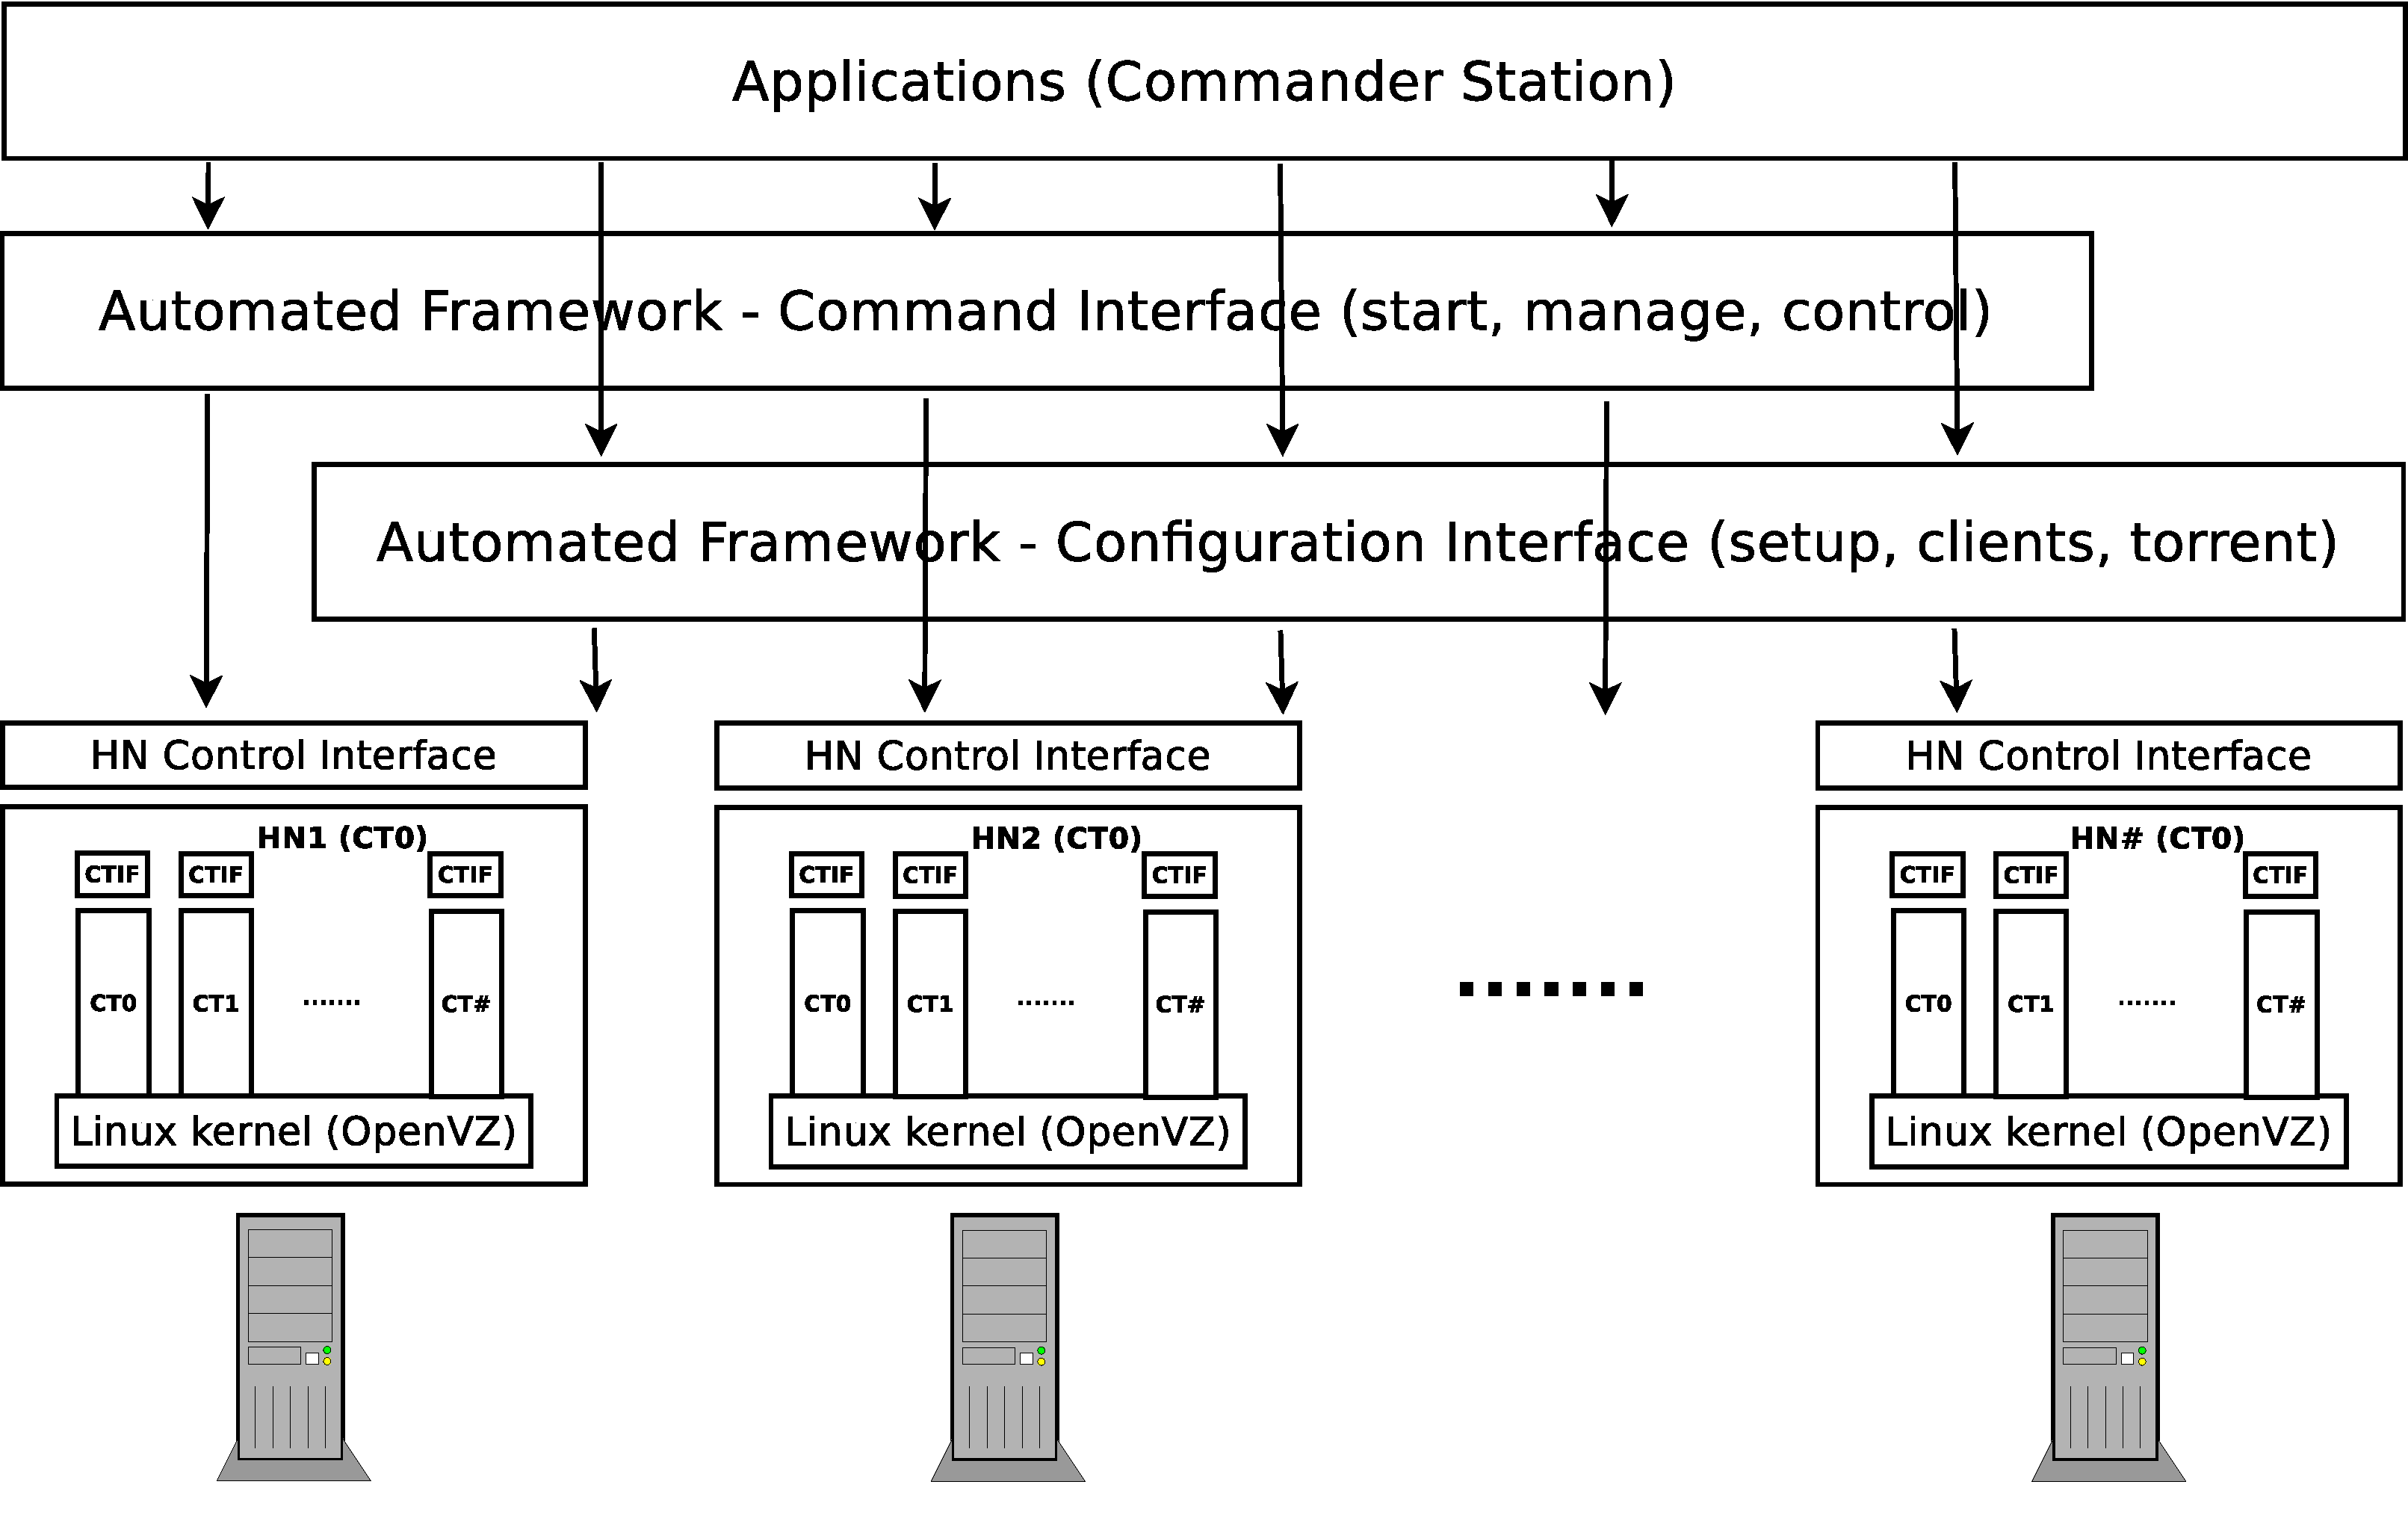
\includegraphics[width=0.7\textwidth]{src/img/virt-infra/virt-infra-overview}
  \end{center}
  \caption{Infrastructure Overview}
  \label{fig:virt-infra:infrastructure-overview}
\end{figure}

Figure~\ref{fig:virt-infra:infrastructure-overview} presents a general
overview of the BitTorrent Testing Infrastructure.

The infrastructure is design to run commodity hardware systems. Each system
uses OpenVZ virtual machine implementation to run multiple virtual systems on
the same hardware node.  Each virtual machine contains the basic tools for
running and compiling the BitTorrent clients. BitTorrent implementations have
been instrumented for automated command and also for outputting status and
logging information required for subsequent analysis and result
interpretation. As the infrastructure aims to be generic among different
implementation, the addition of a new BitTorrent client means adding the
required scripts and instrumentation.

Communication with the virtual machines is enabled through the use of DNAT and
iptables. \texttt{tc} (traffic control) is used for controlling the virtual
links between virtual systems. Each virtual machines uses a set of scripts to
enable the starting, configuration, stopping and result gathering for
BitTorrent clients.

A test/command system can be used to start a series of clients automatically
through the use of a scripted interface. The command system uses SSH to
connect to the virtual machines (SSH is installed and communication is enabled
through DNAT/iptables) and command the BitTorrent implementations. The SSH
connection uses the virtual machines local scripts to configure and start the
clients.

The virtualized environment is thus a cheaper and more flexible alternative to
a full-fledged cluster with little performance loss. Its main disadvantage is
the asymmetry between virtualized environments that run on different hardware
system. The main issue is network bandwidth between VEs running on the same
hardware node and VEs running on different hardware nodes. This can be
corrected by using traffic limitation ensuring a complete network bandwidth
symmetry between the VEs.

\subsection{Virtualized Network Configuration}
\label{sec:virt-netconf}

To simulate real network bandwidth restrictions we use Linux traffic control
(the \texttt{tc} tool) or client-centric options to limit peer upload/download
speed. As virtualized systems are usually NAT-ed, \texttt{iptables} is also
used on the base stations. \texttt{tc} rules are applied both to OpenVZ
containers and to physical systems in order to ensure bandwidth limitation.

As all stations use common scripts and the same BitTorrent clients, important
parts of the filesystem are accessed through NFS (\textit{Network File
System}). Thus, in case of 100 virtualized systems, only one of them is
actually storing configuration, executable and library files; the other
systems use NFS.

Easy system administration has been ensured through the use of
cluster-oriented tools such as \textit{Cluster SSH} or \textit{Parallel SSH}.

As each container runs on top of a hardware node (base system), most
connections use the hardware node as a switch/router. The basic \texttt{venet}
interface allows the container to use the hardware node as a gateway, with the
help of the \texttt{iptables} tool. Connections through the ``hardware node
gateway'' are thus NAT-ed. This poses some configuration overhead as peers
must enable upload slots that must pass through the gateway.

In order to discard the configuration overhead for configuring NAT, a
different approach may be undertaken: the use of \texttt{veth} interfaces and
host bridges. \texttt{veth} interfaces allow the integration of new interfaces
for the containers. \texttt{veth} interfaces may be bridged together using the
\texttt{brctl} on the host system. The host system acts as a switch for
containers. At the same time, all containers, even when residing on different
systems, are able to communicate with each other, as part of the same LAN. All
host systems and the physical interconnecting switch act as a switched network
topology. This makes it very easy to achieve rapid connectivity among peers
running in different OpenVZ containers.

In order to ensure rapid communication of information among containers, NFS
(Network File System) has been employed. NFS is used to share scripts and
repositories among physical systems and among containers. Each update is
instantly available among all systems. Apart from the update improvement,
space is also saved by unifying similar content in a single storage area.

The NFS server is running on one of the base systems/hardware nodes; mount
points are defined on each of the other base systems and on every container. A
specialized \texttt{bin/} folder stores useful scripts for the virtualized
network infrastructure. Various scripts account for various functionalities,
either for the base system or the containers on top of that:

\begin{itemize}
  \item creating and destroying OpenVZ containers;
  \item basic network configuration for each container;
  \item check Internet connectivity for OpenVZ containers;
  \item check container-to-container connectivity using host bridges and
  \texttt{veth} interfaces;
  \item run a command on each container;
  \item copy a file on each container;
  \item apply and test \texttt{tc}-based bandwidth limitation rules.
\end{itemize}

\section{Virtualized Hardware Configuration}
\label{sec:virt-hwconf}

The physical infrastructure is currently hosted in the UPB NCIT
cluster\footnote{\url{http://cluster.grid.pub.ro/}} and
consists of 10 identical hardware systems. A thin OpenVZ virtualization layer
allows easy multiplication of base systems. We are able to safely deploy 100
virtualized systems; most scenarios use a virtual environment as a sandbox for
running a single BitTorrent client. Tools such as \texttt{brctl},
\texttt{iptables} or \texttt{tc} have been employed for ensuring proper
network configuration between virtual environments.

Our current setup consists of 10 computers each running 10 OpenVZ virtual
environments (VEs). All systems are  identical with respect to the CPU power,
memory capacity and HDD space and are part of the same network. The network
connections are 1Gbit Ethernet links.

At the time of this writing, the BitTorrent Testing Infrastructure consists of
8 hardware systems running Debian GNU/Linux 5.0 (Lenny). Any other Linux
distribution can be used as the tools used in the framework are common among
distributions.

The hardware specifications are:

\begin{itemize}
  \item HDD -- SATA Western Digital, WDC WD3000JD-98K, 300GB (279GiB)
  \item Intel Pentium 4 CPU 3.00GHz, dual-core, clock 800MHz, 64 bits
  \item 2GiB RAM, DIMM 533MHz
  \item L1 cache -- 16KiB, L2 cache -- 2MiB
  \item 82545GM Gigabit Ethernet Controller, driver=e1000, speed=1Gbit/s
  \item Motherboard, D2151-A1, FUJITSU SIEMENS
\end{itemize}

All systems are running the same operating system (Debian GNU/Linux
Lenny/testing) and the same software configuration.

With 5 VEs active and running a BitTorrent client, memory consumption is
180MB-250MB per system. With no VE running the memory consumption is around
80MB-110MB. The BitTorrent client used pervasively is
hrktorrent\footnote{\url{http://50hz.ws/hrktorrent/}}, a
libtorrrent-rasterbar\footnote{\url{http://www.rasterbar.com/products/libtorrent/}} based implementation. hrktorrent is a light addition tot
the libtorrent library so memory consumption is quite small while still
delivering good performance. On average each virtual machine uses 40MB of RAM
when running hrktorrent in a BitTorrent swarm.

The current partitioning scheme for each system leaves 220GB of HDD space for
the VEs. However, one could upgrade that limit safely to around 280GB. Each
basic complete VE (that is one with all clients installed) uses 1.7GB of HDD
space. During a 700MB download session, each client outputs around log files
using 30-50MB of space. Processor usage is not an issue as BitTorrent
applications are mostly I/O intensive.

In order to install a new virtual machine, one should use an OpenVZ template
allowing for easy installation. A template contains all basic clients and
tools necessary for running automated tests. The deployment of a new virtual
machine is enabled through the use of the vzctl create command. We recommend
the use of the \texttt{makevz} and \texttt{destroyvz} scripts from the
repository that also configure all necessary aspects for the virtual machines
(hostname, memory, disk space, iptables rules etc.):

\footnotesize
\begin{verbatim}
p2p-next-09:~/bin# ./makevz 106 p2p-next-09-01
Creating VE private area (debian-4.1-amd64-p2p-clean)
Performing postcreate actions
VE private area was created
Saved parameters for VE 1066
Saved parameters for VE 106
Saved parameters for VE 106
Saved parameters for VE 106
Saved parameters for VE 106
Saved parameters for VE 106
Saved parameters for VE 106
Saved parameters for VE 106
Starting VE ...
VE is mounted
Adding IP address(es): 172.16.10.6
Setting CPU units: 1000
Configure meminfo: 131072
Set hostname: p2p-next-09-01
File resolv.conf was modified
VE start in progress...
p2p-next-09:~/bin# vzlist
      VEID      NPROC STATUS  IP_ADDR         HOSTNAME
       101          7 running 172.16.10.1     p2p-next-09-01
       102          7 running 172.16.10.2     p2p-next-09-02
       103          7 running 172.16.10.3     p2p-next-09-03
       104          7 running 172.16.10.4     p2p-next-09-04
       105          7 running 172.16.10.5     p2p-next-09-05
       106          7 running 172.16.10.6     p2p-next-09-06
p2p-next-09:~/bin# ls /home/p2p/ve/
101  102  103  104  105  106
p2p-next-09:~/bin# ./destroyvz 106
Stopping VE ...
VE was stopped
VE is unmounted
Destroying VE private area: /var/lib/vz/private/106
VE private area was destroyed
p2p-next-09:~/bin# vzlist
      VEID      NPROC STATUS  IP_ADDR         HOSTNAME
       101          7 running 172.16.10.1     p2p-next-09-01
       102          7 running 172.16.10.2     p2p-next-09-02
       103          7 running 172.16.10.3     p2p-next-09-03
       104          7 running 172.16.10.4     p2p-next-09-04
       105          7 running 172.16.10.5     p2p-next-09-05
p2p-next-09:~/bin# ls /home/p2p/ve/
101  102  103  104  105
\end{verbatim}
\normalsize

Most OpenVZ functionality is enabled through the use of the \texttt{vzctl}
parent command. Apart from create and destroy subcommands, other commands are
useful:

\begin{itemize}
  \item \texttt{enter $<$veid$>$} -- for entering a virtual machine with the
  \texttt{$<$veid$>$} identifier;
  \item \texttt{start $|$ stop $|$ restart $<$veid$>$} -- for starting,
  stopping or restarting a virtual machine;
  \item \texttt{exec $<$veid$>$ command} -- for executing a certain command on
  a virtual machine;
  \item \texttt{set $<$veid$>$ $[$parameters$]$ -{}-save} -- for altering the
  configuration of a virtual machine.
\end{itemize}

\footnotesize
\begin{verbatim}
p2p-next-09:~/bin# vzctl enter 101
entered into VE 101
p2p-next-09-01:/# hostname
p2p-next-09-01
p2p-next-09-01:/# logout
exited from VE 101
p2p-next-09:~/bin# vzctl exec 101 'ps -ef'
UID        PID  PPID  C STIME TTY          TIME CMD
root         1     0  0 Feb27 ?        00:00:12 init [2]
root       340     1  0 Feb27 ?        00:00:01 /sbin/syslogd
102        346     1  0 Feb27 ?        00:00:00 /usr/bin/dbus-daemon --system
root       353     1  0 Feb27 ?        00:00:00 /usr/sbin/sshd
avahi      360     1  0 Feb27 ?        00:00:00 avahi-daemon: running [p2p-next-09-01.local]
avahi      361   360  0 Feb27 ?        00:00:00 avahi-daemon: chroot helper
root       376     1  0 Feb27 ?        00:00:08 /usr/sbin/cron
root     30709     0  0 09:57 ?        00:00:00 ps -ef
\end{verbatim}
\normalsize

A useful command is \texttt{vzlist}, allowing the listing of all virtual
machines  installed on the hardware node:

\footnotesize
\begin{verbatim}
p2p-next-09:~/bin# vzlist
      VEID      NPROC STATUS  IP_ADDR         HOSTNAME
       101          7 running 172.16.10.1     p2p-next-09-01
       102          7 running 172.16.10.2     p2p-next-09-02
       103          7 running 172.16.10.3     p2p-next-09-03
       104          7 running 172.16.10.4     p2p-next-09-04
       105          7 running 172.16.10.5     p2p-next-09-05
\end{verbatim}
\normalsize

\section{Evaluating Virtualization}

With a plethora of virtualization solutions, a infrastructure for deploying
Peer-to-Peer scenario has to take into account the adequacy of each solution.
Through empirical studies we have chosen OpenVZ as a suitable solution for our
needs, with the lack, however, of a formal evaluation method.

Considering the use of virtualization solutions for our purpose we consider
three important dimensions:

\begin{itemize}
  \item \textbf{efficiency} (scalability) -- how many virtual
  machines/containers may be deployed on a virtual host and allow proper
  simulation of an environment;
  \item \textbf{isolation} -- how well are virtual machines' resources
  separated;
  \item \textbf{reliability} -- how many software crashes happen for a given
  solution; this may be due to implementation or to resourse overuse/abuse.
\end{itemize}

Similar metrics have been proposed by Ismail~et~al.~\cite{virt-metrics}. The
have experimentaly measured and defined overhead, variance and isolation
metrics in virtualization. They had used KVM for testing and experimenting.
Our proposed efficiency metric is similar to their variance metric, while
their isolation metric is mostly concerned with CPU and memory fairness among
various VMs. The variance metric introduced is mainly concerned with the
resources in place used by each virtual machine; the efficiency/scalability
metric introduced by us refers to the number of virtual machines that may be
deployed.

Wood~et~al.~\cite{virt-prof-model} have investigated VMware ESX and Xen and
created an I/O model and profile.

An approach similar to ours was undertaken by
Soltesz~et~al.~\cite{virt-doppel}. They considered Xen and Linux Vservers as
the representatives for para- and paene-virtualization. Their metrics included
performance, isolation and scalability with similar meanings ar to ours.

\textbf{Efficiency} is a sheer measure of deploying large numbers of virtual
machines and containers on top of a given hardware system.
Padala~et~al.~\cite{eval-virt-performance} have shown that OpenVZ possesses a
smaller overhead compared to Xen. However, no formal method has been employed
and their study doesn't take into account other OS-level virtualization
solutions.

A formal measurement for virtualization efficiency/performance should consider
three aspects:

\begin{itemize}
  \item hardware resources;
  \item software implementation (in our case, BitTorrent client
  implementation);
  \item virtualization solution.
\end{itemize}

As such, we formalize efficiency as a function of the three dimensions above:

\begin{align}
Eff & = f(HW, SW, VS)\\
Eff & = f(RAM, HDD, CPU, NET, OS, PS, BT, VS, NVM)\\
Eff &= \frac{VMB}{HNB}
\end{align}

where:

\begin{multicols}{2}
    \begin{itemize}
      \item \texttt{Eff}: efficiency/performance
      \item \texttt{HW}: hardware resources
      \item \texttt{SW}: software implementation
      \item \texttt{VS}: virtualization solution
      \item \texttt{RAM}: system RAM
      \item \texttt{HDD}: I/O space
      \item \texttt{CPU}: processor power
      \item \texttt{NET}: networking features
      \item \texttt{OS}: operating system implementation
      \item \texttt{PS}: basic container processes
      \item \texttt{BT}: BitTorrent implementation
      \item \texttt{NVM}: number of virtual machines
      \item \texttt{VMB}: virtual machine behavior
      \item \texttt{HNB}: hardware node behavior
    \end{itemize}
\end{multicols}

Measuring efficiency must the consider the behavior of the system and how
similar is a container/virtual machine to an actual system. For that one may
take into account resource usage, resource contention, responsiveness. These
may be measured through experimental means and subsequently an empirical
approximate formula, taking into account all above mentioned variables, may be
determined.

\textbf{Isolation} is a means of stating how well is a virtual machine
separated from another virtual machine and from the base system. As OpenVZ VEs
are using the same kernel, it is obvious the isolation value is less than that
of Xen of KVM. Isolation serves as an important dimension for measuring
virtualization solution adequacy. The ability to completely isolate a virtual
machine and properly specify its resource usage allows better resemblance to a
base hardware system.

While we find it difficult to properly formalize isolation we consider
achievable a ``virtualization isolation scale'' in which virtualization
solutions may be compared against each other. A rather relative value than an
absolute one. Thus we consider it safe to state that:

\begin{align}
Iso(normal processes) < Iso(chroot) < Iso(OpenVZ, LXC) < Iso(Xen,KVM)
\end{align}

A careful analysis of virtualization solutions, facilities employed, how well
is separation achieved and resource limitation enforced must be undertaken. It
will allow proper relative scale placing of virtualization solutions.

\textbf{Reliability} must be considered when dealing with a heavily used
infrastructure when evaluating multiple virtualization solutions. In our
experience we have encountered several software problems such as disk
inconsistency, operating system level errors and lack of responsiveness due to
the high (ab)use of hardware resources. Our OpenVZ based infrastructure must
be evaluated. Fortunately, there are a number of well defined and thoroughly
analysed measures such as \textit{failure rate} of \textit{mean distance
between failures} that can be taken into account. These have to consider the
evaluating environment, as with the efficiency dimension:

\begin{align}
Rel & = f(HW, SW, VS)\\
Rel & = f(RAM, HDD, CPU, OS (filesystem), PS, BT, VS, NVM)
\end{align}

Properly defined and evaluated dimensions such as efficiency, isolation and
reliability provide an overall view of virtualization solutions and their
adequacy for our specific purpose. We consider there is no ``silver bullet''
solution but rather one that will provide suitable for a class of necessities.
The weight one maps to each of the dimensions would depend on his/her needs
and environment specifics.

More than this, it may not be feasible (nor possible) to extract a formula
taking into account all input data. Rather consider a numeric value for each
metric and ensure a comparison between these values. Such that one may
conclude that affecting one input variable into one direction (increase or
decrease) will have a certain impact on the metric. This is the similar
approach provided by Ismail~et~al.~\cite{virt-metrics}.

We have experimented both with OpenVZ, LXC and Xen-based environment in order
to create a proper experimental testbed for the above metrics.

In OpenVZ's case, our study focused on efficiency/scalability. Active VEs
running the hrktorrent client use about 70 to 170MB of RAM. This gives a rough
estimate of about $[20 MB; 40 MB]$ memory consumption per VE. The basic system
also uses at most 120MB of RAM.

From the HDD perspective, the basic system can be tuned to use 20GB of space
with no major constraints on the software configuration. Each complete VE able
to run all CLI-based BitTorrent clients uses 1.7GB of space. At the same time,
1GB of space should be left for each system for testing and logging purposes
and 5GB for file transfer and storage. This means that 8GB of space should be
reserved for each VE.

The above values are very lax. A carefully tuned system would manage to use
less resources. However, we aim to show that given these high values, an
average PC could still sustain a significant amount of VEs with little
overhead and resource penalty.

Table~\ref{table:virt-infra:openvz} gives a low limit for the number of OpenVZ
virtual environments able to run on a basic PC. Italic means limitation is due
to RAM capacity, while bold means limitation is due to HDD space.

\begin{table}[ht]
  \centering
  \begin{tabular}{|r|r|r|r|r|r|}
    \hline
     & \multicolumn{5}{|c|}{\textbf{Memory}} \\
    \hline
    \textbf{HDD} & \textbf{1GB} & \textbf{2GB} & \textbf{4GB} & \textbf{8GB} &
    \textbf{16GB} \\
    \hline
    80GB & \textbf{7} & \textbf{7} & \textbf{7} & \textbf{7} &
    \textbf{7} \\
    \hline
    120GB & \textbf{12} & \textbf{12} & \textbf{12} & \textbf{12} &
    \textbf{12} \\
    \hline
    200GB & \textbf{22} & \textbf{22} & \textbf{22} & \textbf{22} &
    \textbf{22} \\
    \hline
    300GB & \textit{22} & \textbf{35} & \textbf{35} & \textbf{35} &
    \textbf{35} \\
    \hline
    500GB & \textit{22} & \textit{47} & \textbf{60} & \textbf{60} &
    \textbf{60} \\
    \hline
    750GB & \textit{22} & \textit{47} & \textbf{91} & \textbf{91} &
    \textbf{91} \\
    \hline
    1TB & \textit{22} & \textit{47} & \textit{97} & \textbf{122} &
    \textbf{122} \\
    \hline
  \end{tabular}
  \caption{Scalability in OpenVZ (Number of Containers)}
  \label{table:virt-infra:openvz}
\end{table}

In case of LXC, we've run a scenario involving the use of the Unix gzip
command, used for file compression. This allowed us to measure both CPU and
hard-disk related values concerned with scalability. Tables below present CPU
usage, I/O operations per second disk busy percentage.

\begin{table}[ht]
  \centering
  \begin{tabular}{@{}rrrrr@{}}
    \toprule
    \textbf{No. containers} & \textbf{Average (\%)} & \textbf{Max (\%)} &
    \textbf{Min (\%)} & \textbf{Time (s)} \\
    \midrule
    2 & 19.2 & 21.3 & 18.7 & 2626 \\
    4 & 39.0 & 44.0 & 35.4 & 2786 \\
    8 & 82.3 & 95.6 & 70.6 & 2401 \\
    \bottomrule
  \end{tabular}
  \caption{LXC CPU Usage for gzip}
  \label{table:virt-infra:lxc-cpu}
\end{table}

\begin{table}[ht]
  \centering
  \begin{tabular}{@{}rrrrr@{}}
    \toprule
    \textbf{No. containers} & \textbf{Average (ops/s)} & \textbf{Max (ops/s)} &
    \textbf{Min (ops/s)} & \textbf{Time (s)} \\
    \midrule
    2 & 41.5 & 104.4 & 17.0 & 2626 \\
    4 & 39.0 & 174.2 & 29.2 & 2786 \\
    8 & 176.6 & 275.4 & 84.6 & 2401 \\
    \bottomrule
  \end{tabular}
  \caption{LXC I/O operatinons for gzip}
  \label{table:virt-infra:lxc-io}
\end{table}

\begin{table}[ht]
  \centering
  \begin{tabular}{@{}rrrrr@{}}
    \toprule
    \textbf{No. containers} & \textbf{Average (\%)} & \textbf{Max (\%)} &
    \textbf{Min (\%)} & \textbf{Time (s)} \\
    \midrule
    2 & 11.8 & 32.3 & 5.3 & 2626 \\
    4 & 26.1 & 65.9 & 12.4 & 2786 \\
    8 & 61.3 & 85.4 & 36.2 & 2401 \\
    \bottomrule
  \end{tabular}
  \caption{LXC Disk Busy for gzip}
  \label{table:virt-infra:lxc-disk}
\end{table}

Experimentation for LXC shows a linear growth of CPU usage and disk
utilization. Memory space is always consumed to maximum available such that it
isn't taken into account. The LXC is able to do linear scaling for a heavily
used application with the possibility of more than linear scaling providing
not all containers are heavily used at the same time.

In case of Xen we've used four virtual machines, each using 256MB of RAM and
running on a single core of the base system. These virtual machines were
running ffmpeg, an application for video conversion. Results of CPU and disk
usage are presented in Table~\ref{table:virt-infra:xen-metrics}.

\begin{table}[ht]
  \centering
  \begin{tabular}{@{}lrrr@{}}
    \toprule
    \textbf{Metric} & \textbf{1 VM} & \textbf{2 VMs} & \textbf{3 VMs} \\
    \midrule
    CPU Usage (\%) & 18.49 & 22.07 & 26.85 \\
    Disk writes (bytes/s) & 1008.11 & 1820.96 & 5074.22 \\
    Running Time (s) & 483 & 908 & 1808 \\
    \bottomrule
  \end{tabular}
  \caption{Xen Metrics for ffmpeg}
  \label{table:virt-infra:xen-metrics}
\end{table}

The evolution of various metrics is slightly over-linear in case of disk usage
and close to linear in case of running time. Xen scaling is similar to LXC in
case of running resource intensive applications such as ffmpeg. However, each
virtual machine uses a predefined value for memory which is generally higher
than an operating system-level virtualization solution due to the new kernel
memory and hypervisor overhead.

The usage of virtualization metrics eases comparison among virtualization
solutions and between use cases of a given solution. One may choose among
various situations where to deploy a virtualization solution and may tune it
to provide the desired outcome. The proposed metrics are difficult to be
written down in a mathematic formula but are best used as comparison. Note
that a solution may be suitable when considering one metric, but unsuitable
when considering the other. The user/experimenter is the one deciding what is
the most relevant aspect to be taken into account.

\section{Automating Deployment and Management of Peer-to-Peer Clients}
\label{sec:virt-infra:auto-deploy}

In order to keep up with recent advances in Internet technology, streaming and
content distribution, Peer-to-Peer systems (and BitTorrent) have to adapt and
develop new, attractive and useful features. Extensive measurements, coupled
with carefully crafted scenarios and dissemination are important for
discovering the weak/strong spots in Peer-to-Peer based data distribution and
ensuring efficient transfer.

On top of the virtualized infrastructure, we developed a framework for
running, commanding and managing BitTorrent swarms. The purpose is to have
access to an easy-to-use system for deploying simple to complex scenarios, make
extensive measurements and collect and analyze swarm information (such as
protocol messages, transfer speed, connected peers).

\textit{The swarm management framework}~\cite{swarm-management} is a service-based infrastructure that
allows easy configuration and commanding of BitTorrent clients on a variety of
systems. A client application (\textit{commander}) is used to send
commands/requests to all stations running a particular BitTorrent client. Each
station runs a \textit{dedicated service} that interprets the requests and
manages the local BitTorrent client accordingly.

The framework is designed to be as flexible and expandable as possible. As of
this point it allows running/testing a variety of scenarios and swarms. Based
on the interest of the one designing and running the scenario, one may
configure the BitTorrent client implementation for a particular station, alter
the churn rate by configuring entry/exit times in the swarm, add rate limiting
constraints, alter swarm size, file size etc. Its high reconfigurability
allows one to run relevant scenarios and collect important information to be
analyzed and disseminated.

Through automation and client instrumentation the management framework allows
rapid collection of status and logging information from BitTorrent clients.
The major advantages of the framework are:

\begin{itemize}
  \item \textit{automation} -- user interaction is only required for starting
  clients and investigating their current state;
  \item \textit{complete control} -- the swarm management framework allows the
  user/experimenter to specify swarm and client characteristics and to define
  the context/environment where the scenario is deployed;
  \item \textit{full client information} -- instrumented clients output
  detailed information regarding the inner protocol implementation and
  transfer evolution; information is gathered from all clients and used for
  subsequent analysis.
\end{itemize}

Depending on the level of control of the swarm, we define two types of
environments. A \textit{controlled environment}, or \textit{internal swarm}
uses only instrumented controlled clients. We have complete control over the
network infrastructure and peers. A \textit{free environment} or
\textit{external swarm} is usually created outside the infrastructure, and
consists of a larger number of peers, some of which are the instrumented
controlled clients. Our experiments so far have focused on \textit{controlled
environments}; we aim to extend our investigations to \textit{free environment
swarms}.

\section{Instrumenting Peer-to-Peer Clients}
\label{sec:deploy-instr}

For our experiments~\cite{bt-pef} we selected the BitTorrent clients that are most
significant nowadays, based on the number of users, reported performance,
features and history.

We used Azureus, Tribler, Transmission, Aria, libtorrent rasterbar/hrktorrent,
BitTornado and the mainline client (open source version). All clients are open
source as we had to instrument them to use a command line interface and to
output verbose logging information.

\textbf{Azureus}, now called Vuze, is a popular BitTorrent client written in
Java. We used Azureus version 2.3.0.6. The main issue with Azureus was the
lack of a proper CLI that would enable automation. Though limited, a ``Console
UI'' module enabled automating the tasks of running Azureus and gathering
download status and logging information.

\textbf{Tribler} is a BitTorrent client written in Python and one of the most
successful academic research projects. Developed by a team in TU Delft,
Tribler aims at adding various features to BitTorrent, increasing download
speed and user experience. We used Tribler 4.2. Although a GUI oriented
client, Tribler offers a command line interface for automation. Extensive
logging information is enabled by updating the value of a few variables.

\textbf{Transmission} is the default BitTorrent client in the popular Ubuntu
Linux distribution. Transmission is written in C and aims at delivering a good
amount of features while still keeping a small memory footprint. The version
we used for our tests was transmission 1.22. Transmission has a fully
featured CLI and was one of the clients that were very easy to automate.
Detailed debugging information regarding connections and chunk transfers can
be enabled by setting the TR\_DEBUG\_FD environment variable.

\textbf{Aria2} is a multiprotocol (HTTP, FTP, BitTorrent, Metalink) download
client. Throughout our tests we used version 0.14. aria2 natively provides a
CLI and it was easy to automate. Logging is also enabled through CLI
arguments. Aria2 is written in C++.

\textbf{libtorrent rasterbar/hrktorrent} is a BitTorrent library written in
C++. It is used by a number of BitTorrent clients such as Deluge, BitTorrent
and SharkTorrent. As we were looking for a client with a CLI we found
hrktorrent to be the best choice. hrktorrent is a lightweight implementation
over libtorrent-rasterbar and provides the necessary interface for automating
a BitTorrent transfer, although some modifications were necessary. Rasterbar
libtorrent provides extensive logging information by defining the
TORRENT\_LOGGING and TORRENT\_VERBOSE\_LOGGING\_MACROS. We used version 0.13.1
of libtorrent-rasterbar and the most recent version of hrktorrent.

\textbf{BitTornado} is an old BitTorrent client written in Python. The reason
for choosing it to be tested was because of a common background with Tribler.
However, as testing revealed, it had its share of bugs and problems and it was
eventually dropped.

\textbf{BitTorrent Mainline} is the original BitTorrent client written by Bram
Cohen in Python. We used version 5.2 during our experiments, the last
open-source version. The mainline client provides a CLI and logging can be
enabled through minor modifications of the source code.

\section{Framework Setup}
\label{sec:deploy-fwork}

\begin{figure}[h]
  \begin{center}
    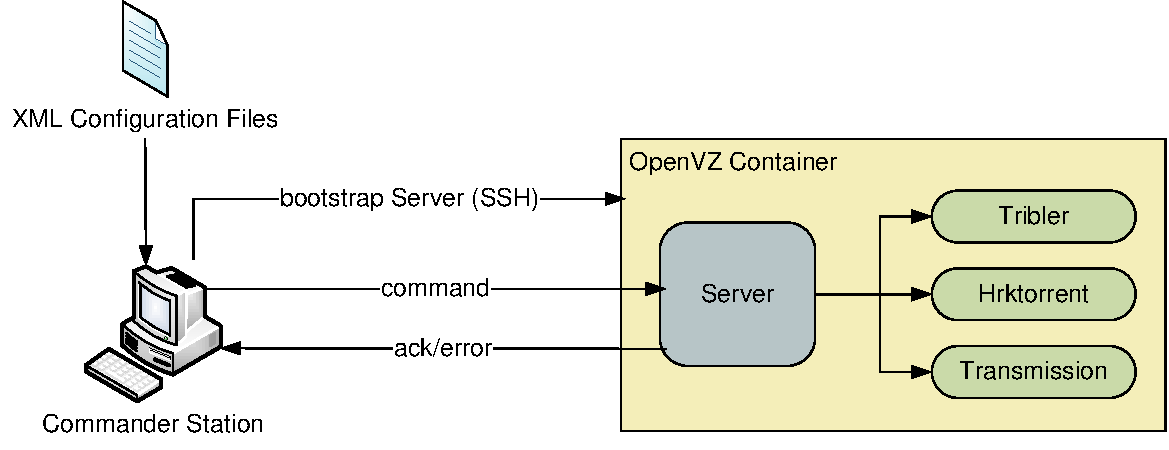
\includegraphics[width=0.7\textwidth]{src/img/virt-infra/service-arch}
  \end{center}
  \caption{Software Service System Overview}
  \label{fig:virt-infra:service-arch}
\end{figure}

The software service infrastructure was designed with the goal of remotely
controlling BitTorrent clients. Its architecture (see
Figure~\ref{fig:virt-infra:service-arch}) is built on a client-server model,
with a single client addressed as \textit{Commander} and multiple servers. The
BitTorrent clients reside in OpenVZ virtual containers and are controlled only
through the \textit{Server} service, by interacting with the Commander
interface. A SSH connection is used by the Commander for the initial
bootstrapping, in case the service is not active.

The BitTorrent scenarios are defined using XML configuration files which can
be considered as input to the Commander. These files contain information not
only about each container that should be used, but also about the torrent
transfers, like file names and paths.

As we wanted to make it as easy as possible to deploy new BitTorrent swarms,
we designed our architecture to support two XML configuration files: one for
physical nodes configuration and one for BitTorrent swarms configuration.

The \textit{nodes} XML file describes the physical infrastructure
configuration. It stores information about:

\begin{itemize}
 \item physical nodes/OpenVZ containers IP addresses and NAT ports;
 \item SSH port and username;
 \item server and Bittorrent clients paths.
\end{itemize}

\scriptsize
\begin{verbatim}
   <node id="1">
     <public_address>141.85.224.201</public_address>
     <public_port>10169</public_port>
     <public_iface>eth0</public_iface>
     <private_address>141.85.224.201</private_address>
     <private_port></private_port>
     <private_iface></private_iface>
     <ssh_port>10122</ssh_port>
     <username>p2p</username>
     <listen_port>10104</listen_port>
     <daemon_dir>/home/p2p/cs-p2p-next/autorun/server/</daemon_dir>
     <daemon_file>Server.py</daemon_file>
     <clients>
       <client id="transmission">
         <base>/home/p2p/p2p-clients/transmission/cli</base>
       </client>
       <client id="hrktorrent">
         <base>/home/p2p/p2p-clients/hrktorrent</base>
       </client>
       <client id="tribler">
         <base>/home/p2p/p2p-clients/tribler</base>
       </client>
     </clients>
   </node>
\end{verbatim}
\normalsize

The \textit{swarm} XML file is used to describe the swarm configuration. It
maps a BitTorrent client to a physical node from the nodes XML configuration
file, and contains the following information:

\begin{itemize}
  \item torrent file for the experiment (same path on all containers);
  \item BitTorrent client upload/download speed limitations;
  \item output options (download path, logs paths).
\end{itemize}

The speed limitations are enforced using the \textit{tc} Linux tool or
internal client bandwidth limitation options.

\scriptsize
\begin{verbatim}
 <swarm>
   <torrent_file>/home/p2p/p2p-meta/test.torrent</torrent_file>
   <instance id="1">
     <node>1</node>
     <client>tribler</client>
     <upload_limit>512</upload_limit>
     <download_limit>256</download_limit>
     <download_dir>/home/p2p/p2p-dld/tribler</download_dir>
     <log_dir>/home/p2p/p2p-dld/tribler</log_dir>
     <log_file>tribler-test.log</log_file>
     <output_dir>/home/p2p/p2p-log/tribler</output_dir>
     <output_file>tribler-test.out</output_file>
     <actions/>
   </instance>
 <swarm>
\end{verbatim}
\normalsize

\section{Client Startup and Management}
\label{sec:deploy-startup}

The \textit{Server} application represents a daemon that listens for incoming
connections and manages BitTorrent clients. Upon start-up, the server receives
as input from the Commander the IP address on which to bind itself for socket
connections. The port on which it listens is predefined in a configuration
file visible to both Server and Commander.

Similar to the Commander application, the language chosen for the
implementation is Python, which offers several C-like functionalities, like
the \textit{socket} module for communication and the \textit{subprocess} for
process spawning (the server is responsible for starting and stopping the
BitTorrent clients). The BitTorrent swarm analysis system described in
Section~\ref{sec:proto-measure:data-processing} is also entirely implemented
in Python, and the Server uses its status file parsers in order to obtain the
latest information about a transfer status.

The Server is separated from the BitTorrent clients using a thin layer of
classes, implemented for each client, which provide the interface needed for
commanding their execution and establishing their input parameters.

The system design implies that BitTorrent clients reside on remote machines
and are managed through a \textit{Server} application, which runs as a daemon
on their system. This Server is remotely controlled, being started, restarted
and stopped using SSH commands initiated through the \textit{Commander}
application. Once the Server is started, the Commander acts as its client,
communicating with it in order to control the BitTorrent applications. Our
protocol implies that each BitTorrent client started by the Server is
associated with only one torrent file.

Currently, the software service infrastructure supports the following messages:
\begin{itemize}
  \item \textit{START-CLIENT} -- the server will start a client with the given
  parameters;
  \item \textit{STOP-CLIENT} -- the server will stop a client with the given
  identifier;
  \item \textit{GET-CLIENTS} -- the server replies with a list of running
  clients;
  \item \textit{GET-OUTPUT} -- the server replies with information about
  clients output (running or not);
  \item \textit{ARCHIVE } -- the server creates archives with the files
  indicated in the message, and deletes the files;
  \item \textit{GET-STATUS} - returns information about an active transfer;
  \item \textit{CLEANUP} - removes files, extendible to other file types.
\end{itemize}

The dictionary maps the types of the files that need to be removed, in the
current version of the implementation it supports the following keys:

\begin{itemize}
  \item ALL -- if True, erases all files related to the experiment;
  \item DOWN -- if True, erases all downloaded files;
  \item VLOGS -- if True, erases all verbose log files;
  \item SLOGS -- if True, erases all status log files;
  \item ARCHIVE -- if True, erases all archives related to the experiment.
\end{itemize}

The Commander initiates transfers by starting a client with a specific torrent
file and options (download path, log files paths and names), and the Server
returns a corresponding ID, which can be used to check the transfer status.
The \textit{status information} is retrieved from the status log files, and
currently supports the following parameters: download speed, upload speed,
downloaded size, uploaded size, eta (estimated time of arrival), number of
peers. In the reply message body, each parameter uses a string identifier
(parameter_name) and is followed by its corresponding value.

The use-cases involved swarms with different numbers of peers on torrent files
of different sizes (ranging from tens of MB to a few GB for Linux distribution
ISO files). In a typical scenario, the Commander loads the XML configuration
files representing the swarm and then it bootstraps the Server daemons from
all the virtual containers. Immediately afterwards, the Commander uses the
Server daemons to start BitTorrent clients on a target torrent. Once the swarm
is formed, the Commander then periodically checks the state of the BitTorrent
clients in the swarm. It also stops/restarts some of the clients.

The logs generated by the BitTorrent clients contain lines of the following
form:

\begin{itemize}
  \item Hrktorrent status log:\\
  \textit{ ps: 32, dht: 21 $<>$ time: 17-08-2010 12:40:05 $<>$ dl: 2.57kb/s,
  ul: 3.09kb/s $<>$ dld: 0mb, uld: 0mb, size: 3125mb $<>$ eta: 5d 46h 23m 8s}
  \item Tribler status log:\\
  \textit{03-06-2010 12:19:04 sample1.mpeg DLSTATUS_DOWNLOADING 93.89\% None
  up 0.00KB/s down  5440.21KB/s eta 1.67072531777 peers 2}
  \item Hrktorrent verbose log:\\
  \textit{Jun 08 22:20:48 $<==$ HAVE [ piece: 839]}
  \item Tribler verbose log:\\
  \textit{14-11-2009 23:11:13 connecter: Got HAVE( 14 ) from 141.85.37.41}
\end{itemize}

\section{Simulating Connection Dropouts}
\label{sec:virt-infra:dropouts}

In order to create a realistic behavior of a Peer-to-Peer swarm, the
experimenter must take into account the way connections are created and then
destroyed; in other terms, churning must be considered. We define simulating
churn as \textit{simulating connection dropouts}~\cite{simulating-dropouts}.
These techniques have to be taken into account to provide valuable updates to
the virtualized network infrastructure.

We analyse two solutions for reproducing realistic network
dropouts in simulation environments and compare them with an induced network
failure. Considering infrastructures where complete control exists over the
client processes and machines, the peer connections to the swarm are dropped
and resumed by stopping and restarting the client, suspending and resuming the
client and disabling and enabling the network interface. The client behavior
in the first two solutions is compared to the third network dropout solution
from the swarm's point of view.

\subsection{Reproducing Network Behavior}
\label{subsec:virt-infra:behavior}

One of the main difficulties in simulating network environments is reproducing
network unreliability. Given the heterogeneous nature of both end-user
computers and ISP equipments and policies, a real-life deployment of
Peer-to-Peer systems encounters multiple types of underlying network issues:
dropped packages, connection delays, connection dropouts.

Each of the above mentioned network behaviors may have an influence on
application behavior. If connection delays and dropped packages are most of
the times covered by TCP functionality, connection dropouts have a direct
influence on the application level (clients joining and leaving are a
fundamental process of Peer-to-Peer system~\cite{p2p-file-sharing-workload}).
Considering one simple example of a swarm composed of an initial seeder and
six leechers, if the seeder periodically leaves and rejoins the swarm, the
nodes will require a longer period of time for the data transfer to be
completed.

BitTorrent clients create and maintain reputation traces for peers with
whom data was exchanged. In case a peer possesses an unreliable behavior, it
will not be preferred for opening new connection slots and thus it will
experience a decreased level of performance from the rest of the swarm.

Connection dropouts also contribute to peer population
churn~\cite{understanding-churn}. As nodes are disconnected from the swarm, the
rest of peer population may have an improved or diminished performance,
depending on the swarm state. Previous studies have estimated and analysed the
impact of churn on the behavior of Peer-to-Peer
protocols~\cite{Binzenhofer:2007:ECS:1769187.1769257}. However, in most cases,
the analysis was based on simulations of protocols (\cite{Luo2010},
\cite{Katsaros2009}, \cite{Ou:2010:PEK:1749614.1749649}) rather than using
real implementations.

From the point of view of the swarm, a client connection dropout is equivalent
to the client abruptly leaving the system. In this case neither the
BitTorrent connections, nor the TCP links are closed in a graceful manner and
swarm peers will experience multiple timeouts before declaring the connections
closed.

Such behavior can be reproduced using three solutions: stopping and restarting
the clients, suspending them and disabling the network interface.

Clients can be instantly stopped using the POSIX SIGKILL signal. When a
process receives this signal, it is immediately stopped and all its open
connections are closed by the operating system. In order for the client to be
resumed, it has to be restarted.

When a process is suspended, it is placed in a temporary inactive state. The
operating system does not close its connections and open files. A process
can easily be suspended by sending it a POSIX SIGSTOP signal. To resume the
process (and place it in an active state), the POSIX SIGCONT signal has to be
sent to the process.

The solutions for separating the client from the swarm are different from the
point of view of the TCP connection management: the stopped clients have all
their connections closed, while the suspended clients can resume their
connections if a timeout has not been reached at the moment of their resume.

The client connection dropout can be induced by disabling the network
interface. Using this approach the client will continue to run without any
intervention from the operating system while its TCP connections will be
closed. Disabling the network interface closely reproduces network dropouts
occurring in the Internet.

\subsection{Experimental Setup}
\label{subsec:virt-infra:dropouts-setup}

Practical demonstration and evaluation of the connection dropout features
have employed the virtualized infrastructure and shte scripted framework
running on top of it. The infrastructure allowed us to deploy up to 80 peers
-- each running in a single virtual machine. All peers have been grouped in
pairs to evaluate proposed solutions for simulating connection dropout
features. The thin scripted framework was also responsible for collecting
output from all peers (in the form of log files) and for parsing it.

The infrastructure is constructed on top of several commodity hardware systems
in the NCIT cluster from UPB. In order to
deploy a large number of peers, the thin virtualization layer employed OpenVZ.
OpenVZ is a lightweight solution that allows rapid creation of
virtual machines (also called containers). As an operating system-level
virtualization solution, OpenVZ enables creation of a large number of virtual
machines (30 virtual machines are sustainable on a system with 2GB of RAM
memory). In our infrastructure each container is running a single BitTorrent
client instance.

All hardware systems used were identical with respect to hardware and software
components: 2GB RAM, 3 GHz dual-core CPU, 300GB HDD, 1Gbit NIC, running Debian
GNU/Linux 5.0 Lenny. The deployed experiments used a single OpenVZ container
for each peer taking part in a swarm. The virtualized network
allowed a direct link layer access between systems -- all systems are part of
the same network; this allows easy configuration and interaction.

A separate hardware system, also called Commander, was used to start and
handle scenarios. The Commander uses SSH for communicating with the
virtualized environment. Connections between Commander and containers are
handled through secondary specialized \texttt{venet} interfaces; the presence
of the Commander connections and the virtualized network created an easy
testing ground for disabling and enabling interfaces -- the interfaces
employed for dropping connections were those part of the virtualized network.

The experiments made use of an updated version of hrktorrent, a lightweight
application built on top of libtorrent-rasterbar. Previous
experiments~\cite{bt-vi} have shown libtorrent-rasterbar outperforming other
BitTorrent implementations leading to its usage in the current experiments.
The hrktorrent has been updated to make use of bandwidth limitation facilities
provided by libtorrent-rasterbar.  Deployed scenarios have forced a 100 KB/s
download limit.

To evaluate the impact of the dropout, clients have been grouped into pairs
(one seeder and one leecher), the leecher's downloading capacity being
temporary disabled. Together with the seeder and leecher, a tracker is started
on the same container as the seeder to allow BitTorrent communication between
the two nodes. The use of a two-peer swarm reduces the impact of
non-deterministic BitTorrent communication inside the swarm. At the same time,
this setup emphasizes the activity of the target leecher by clearly targeting
one BitTorrent connection. Placing the tested leecher in a larger swarm would
make the results less accurate.

The duration of the download has to be large enough to allow the experiments
to avoid the BitTorrent-specific start-up behavior. Given the leecher's
bandwidth limitation of 100 KB/s, a 100MB file was chosen to be shared by the
seeder. This creates a theoretical duration of 1000 seconds for each complete
download. However, the size of the shared files has no effect on the
connection dropout behavior: the leecher's bandwidth will always be saturated
at the moment of the dropout simulation.

Time recovery is the interval of inactivity of a given peer and, thus, of a
connection between two peers. Through various methods, the connection between
peers is disabled and, after a given period of time, reenabled. Time recovery
is the focus of our experiments and may on may not differ significantly from
the connection interrupt timeout. The connection behavior of each of these
methods provides insight on their suitability for various simulation
scenarios.

Each seeder-leecher pair is executing the following scenario schedule:

\begin{itemize}
  \item start tracker, create .torrent files
  \item start seeder, leecher
  \item wait a predetermined amount of time for swarm initialization
  \item disable the leecher, in accordance to the respective connection
  dropout solution (suspend the process, terminate it or disable the network
  interface)
  \item wait a test-specific amount of time
  \item enable the leecher
  \item wait for swarm stabilization
\end{itemize}

The amount of time before the leecher is disabled and after it is enabled
have been used to ensure swarm stabilization and proper results. At this
point, the ``swarm initialization time'' is 15 seconds, while the ``swarm
stabilization time'' is 45 seconds. These time intervals have been chosen
empirically from experimentation and experience. A thorough analysis of the
optimum values for the time intervals is set as further work.

A leecher-seeder pair is terminated after each scenario and restarted in order
to take part in the next one. A complete test suite for a given pair implies
using increasing amounts of timeout between disabling and enabling the
leecher. This is, for every situation, equivalent to an increase in the
duration of the connection dropout and forms the basis for subsequent
analysis. The values chosen for timeout intervals are measured in seconds in
geometric progression: 4 seconds, 8 seconds, 16 seconds, 32 seconds, 64
seconds, 128 seconds, 256 seconds, 512 seconds. They cover a simulated dropout
timeout ranging from a few seconds to close to 10 minutes.

\subsection{Results}
\label{subsec:virt-infra:results-dropouts}

The virtualized infrastructure and scripted framework have been used as an
evaluation suite testing-ground for the proposed dropout equivalent solutions.
The evaluation suite has employed virtualized containers to create
leecher-seeder pairs.

Each pair is used to transfer a 100 MB file from an initial seeder to one
leecher. A tracker is also started on the same container as the seeder to
mediate communication. The leecher uses a 100 KB/s limitation. Information
from both the leecher and the seeder is collected as log files and parsed
subsequently.

The accessibility of a high number of virtualized systems and the small swarm
size (two peers, one leecher and one seeder) allows rapid deployment of
scenarios and easy repeatability. A single running suite employs 39 swarm
pairs, 13 pairs for each proposed solution. Through the scripted interface
each pair is sequentially simulating a series of connection dropouts. Each
series consists of dropping the connection for 4 seconds, 8 seconds, 16
seconds and so on until 512 seconds. A simulated dropout is equivalent to a
connection interrupt for the given amount of time.

Information used for analysis has been collected in the form of log files from
BitTorrent clients. SSH, rsync and shell scripts have been glued together in
order to collect and parse relevant information. Statistical processing has
been employed in the form of R language scripts for mean values, standard
deviation, graphics, etc.

The main goal of the employed experiments is to measure and compare the
recovery time after each connection drop out for each of the three proposed
solutions. By employing diverse timeout intervals we present similarities and
differences between suspending and terminating clients or disabling network
interfaces in order to simulate connection dropout.

% ifdown, mean and rsd
\def \meanifa {0}
\def \rsdifa {0}
\def \meanifb {12.10}
\def \rsdifb {10.88}
\def \meanifc {23.84}
\def \rsdifc {16.73}
\def \meanifd {47.16}
\def \rsdifd {4.50}
\def \meanife {79.66}
\def \rsdife {13.4}
\def \meaniff {146.37}
\def \rsdiff {8.05}
\def \meanifg {288.58}
\def \rsdifg {2.15}
\def \meanifh {535.42}
\def \rsdifh {0.09}

% suspend, mean and rsd
\def \meansuspenda {0}
\def \rsdsuspenda {0}
\def \meansuspendb {9.80}
\def \rsdsuspendb {4.30}
\def \meansuspendc {17.12}
\def \rsdsuspendc {2.33}
\def \meansuspendd {32.33}
\def \rsdsuspendd {8.87}
\def \meansuspende {72.16}
\def \rsdsuspende {26.83}
\def \meansuspendf {142.11}
\def \rsdsuspendf {11.56}
\def \meansuspendg {259.90}
\def \rsdsuspendg {1.56}
\def \meansuspendh {532.42}
\def \rsdsuspendh {2.11}

% stop, mean and rsd
\def \meanstopa {0}
\def \rsdstopa {0}
\def \meanstopb {12.21}
\def \rsdstopb {11.61}
\def \meanstopc {19.95}
\def \rsdstopc {9.04}
\def \meanstopd {36.36}
\def \rsdstopd {4.11}
\def \meanstope {67.61}
\def \rsdstope {2.45}
\def \meanstopf {131.80}
\def \rsdstopf {1.14}
\def \meanstopg {260.26}
\def \rsdstopg {0.69}
\def \meanstoph {515.81}
\def \rsdstoph {0.33}


%\begin{sidewaystable}
\begin{table}
  \centering
  \caption{Recovery Timeout for Different Scenarios}
  \label{tab:virt-infra:recovery}
  \begin{tabular}{@{}rrrrrrr@{}}
    \toprule
      & \multicolumn{2}{c}{\textbf{ifdown}} & \multicolumn{2}{c}{\textbf{suspend}} & \multicolumn{2}{c}{\textbf{stop}} \\
    \cmidrule{2-3} \cmidrule{4-5} \cmidrule{6-7}
      \textit{pause(s)} & \textit{mean(s)} & \textit{rsd(\%)} & \textit{mean(s)} & \textit{rsd(\%)} & \textit{mean(s)} & \textit{rsd(\%)} \\
    \midrule
%      4 & \meanifa & \rsdifa & \meansuspenda & \rsdsuspenda & \meanstopa &
%      \rsdstopa \\
      8 & \meanifb & \rsdifb & \meansuspendb & \rsdsuspendb & \meanstopb &
      \rsdstopb \\
      16 & \meanifc & \rsdifc & \meansuspendc & \rsdsuspendc & \meanstopc &
      \rsdstopc \\
      32 & \meanifd & \rsdifd & \meansuspendd & \rsdsuspendd & \meanstopd &
      \rsdstopd \\
      64 & \meanife & \rsdife & \meansuspende & \rsdsuspende & \meanstope &
      \rsdstope \\
      128 & \meaniff & \rsdiff & \meansuspendf & \rsdsuspendf & \meanstopf &
      \rsdstopf \\
      256 & \meanifg & \rsdifg & \meansuspendg & \rsdsuspendg & \meanstopg &
      \rsdstopg \\
      512 & \meanifh & \rsdifh & \meansuspendh & \rsdsuspendh & \meanstoph &
      \rsdstoph \\
    \bottomrule
  \end{tabular}
\end{table}
%\end{sidewaystable}


Table~\ref{tab:virt-infra:recovery} summarizes the results of the employed
experiments.  The three main methods used for simulating connection dropouts
are identified by \textbf{ifdown}, \textbf{suspend} and \textbf{stop}. For
each method, the mean value of the recovery timeout and the relative standard
deviation have been computed. The column dubbed \textit{pause} signifies the
timeout implied on the given process. The \textit{mean} column is the mean of
the measured values, measured in seconds, while the \textit{rsd} column is the
relative standard deviation (percentage).

All three methods offer similar results, with recovery time values closer
as the scheduled pause time increases. The \textbf{suspend} and \textbf{stop}
are usually very close to the real \textbf{pause} value, while the
\textbf{ifdown} method is usually further from that value. Due to their
similar results, we consider safe to assume that the \textbf{suspend} and
\textbf{stop} methods may be used interchangeably in order to simulate
connection dropouts. As a connection dropout is usually caused by a client
process being terminated, the \textbf{stop} method is the most appropriate
choice. If available or easier to deploy, the \textbf{suspend} method may be
used with similar effects.

Figure~\ref{fig:virt-infra:time-recovery} shows a graphical representation of
the recovery time for the solutions involving interface disable and
terminating the process with respect to the leecher timeout interval. We have
found the results regarding suspending the process to be inconclusive due to
improper swarm initialization time and have been left out.

\begin{figure}[h]
  \begin{center}
    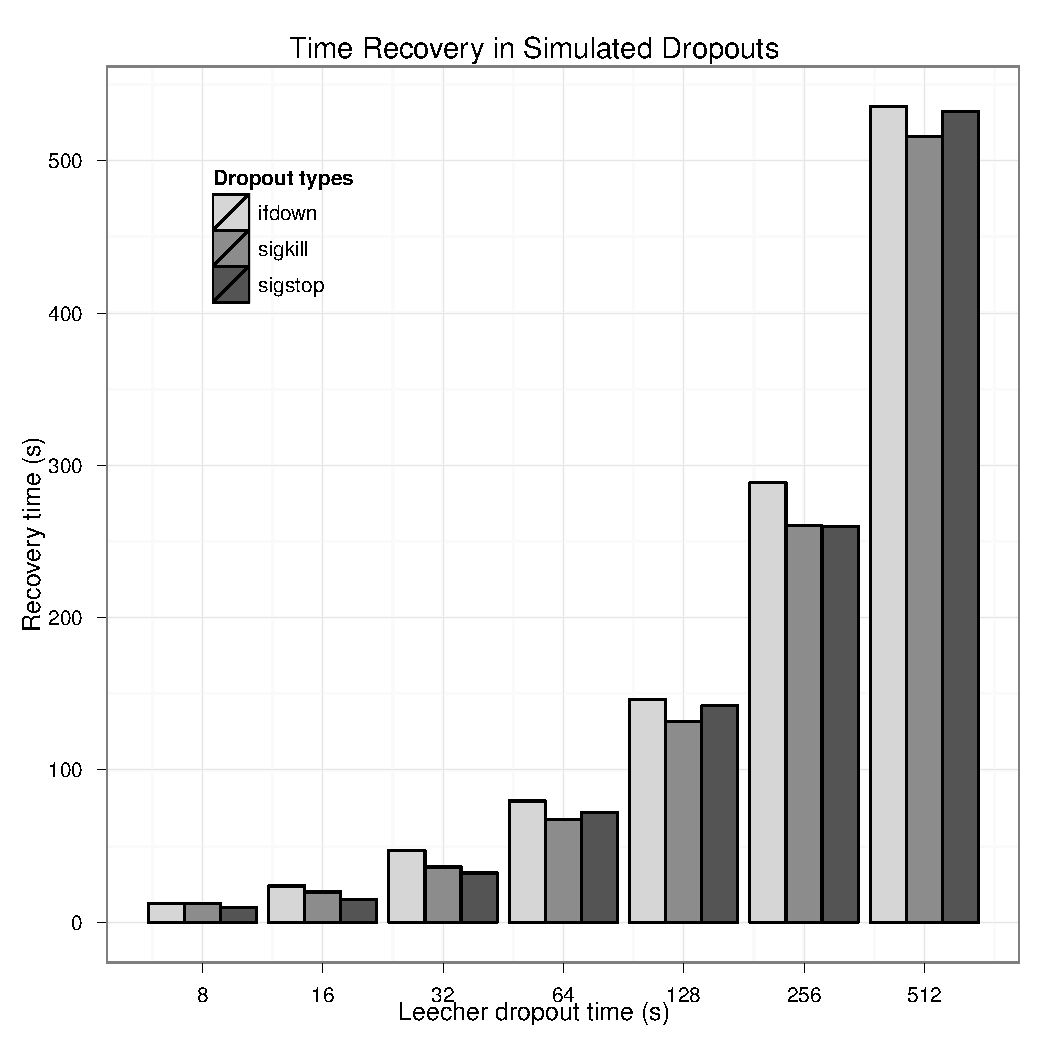
\includegraphics[width=0.5\textwidth]{src/img/virt-infra/recovery-in-simulated-dropouts.pdf}
  \end{center}
  \caption{Time Recovery with Respect to Dropout Interval}
  \label{fig:virt-infra:time-recovery}
\end{figure}

As concluding remarks, the first solution (\textbf{ifdown}) brings down the
network interface of the peer in order to simulate the end of the connection.
Results have shown that recovery time, although in the same range, is higher
than the other methods and we conclude that such a solution would be mostly
suitable for simulating connection dropouts due to network failure.

The second solution (\textbf{suspend}) suspends clients during the simulated
dropout (using SIGSTOP) and resumes them afterwards (using SIGCONT). Although
suspending peers is not a common action, results have shown that this method
is similar to the \textbf{stop} method with respect to recovery time. In an
environment where suspending peers is easier to be achieved than stopping them,
such a solution could prove suitable and provide realistic results.

The third solution (\textbf{stop}) consists of stopping (using SIGKILL) and
restarting the clients. This solution (although aggressive) is considered to
be the best approximation of a realistic behaviour of a connection dropout, as
peers have typically high dynamics when entering and exiting a swarm.

\section{Deployed Setup and Experimental Scenarios}
\label{sec:virt-infra:setup-scenarios}

The complete infrastructure, using automation, virtualization, connection
dropout simultion, allows the automatic deployment and management of a wide
variety of Peer-to-Peer scenarios. Each OpenVZ virtualized hosts runs a single
BitTorrent client (or tracker) and collects relevant information for
subsequent analysis. The commander station defines the configuration of the
new scenario and then deploys it on top of the virtualized infrastructure.
Bandwidth limitation, client types, ports to be used, churn rate, torrent
files are setup for the given scenario.

\subsection{Virtualized Configuration}

Our current setup consists of 10 computers each running 10 OpenVZ virtual
environments (VEs). All systems are  identical with respect to the CPU power,
memory capacity and HDD space and are part of the same network. The network
connections are 1Gbit Ethernet links.

At the time of this writing, the BitTorrent Testing Infrastructure consists of
8 hardware systems running Debian GNU/Linux 5.0 (Lenny). Any other Linux
distribution can be used as the tools used in the framework are common among
distributions.

With 5 VEs active and running a BitTorrent client, memory consumption is
180MB-250MB per system. With no VE running the memory consumption is around
80MB-110MB. The BitTorrent client used pervasively is hrktorrent, a
libtorrrent-rasterbar based implementation. hrktorrent is a light addition tot
the libtorrent library so memory consumption is quite small while still
delivering good performance. On average each virtual machine uses 40MB of RAM
when running hrktorrent in a BitTorrent swarm.

The current partitioning scheme for each system leaves 220GB of HDD space for
the VEs. However, one could upgrade that limit safely to around 280GB. Each
basic complete VE (that is one with all clients installed) uses 1.7GB of HDD
space. During a 700MB download session, each client outputs around log files
using 30-50MB of space. Processor usage is not an issue as BitTorrent
applications are mostly I/O intensive.

Experiments unsing a large number of peers have been employed using the
virtualized infrastructure. These experiments use virtualized peers to deploy
realistic swarms, create a network topology and overlay and collect
information for analysis.

\subsection{Monitoring Experiment}

One such experiment simulates swarms comprising of a single seeder and 39
initial leechers. 19 leechers are high bandwidth peers (512KB/s download
speed, 256KB/s upload speed) and 20 leechers are low bandwidth peers (64KB/s
download speed, 32KB/s upload speed).

The total time of an experiment involving all 40 peers and a 700MB CD image
file is around 4 hours. It only takes about half an hour for the high
bandwidth clients to download it.

We have been using Linux Traffic Control (\texttt{tc}) tool combined with
iptables set-mark option to limit download and upload traffic to and from a
VE.

\begin{figure}
  \centering
  \begin{minipage}{0.8\textwidth}
    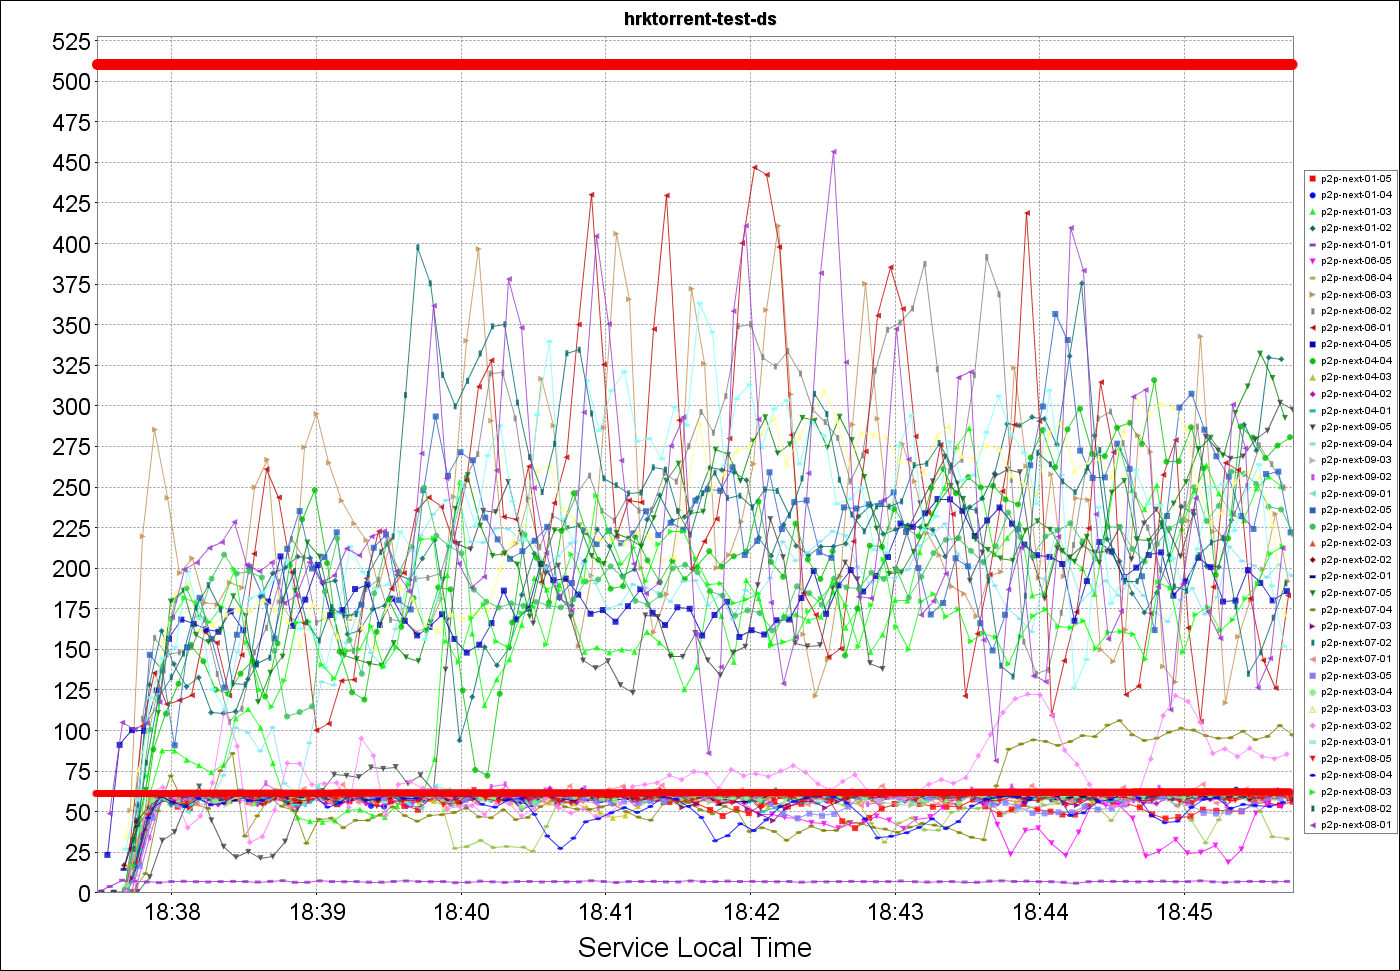
\includegraphics[width=\textwidth]{src/img/virt-infra/test-monalisa-virt-env-start.png}
    \caption{Download Speed Evolution -- Start Phase}
    \label{fig:virt-infra:mon-down-ini}
    \vspace{0.2cm}
    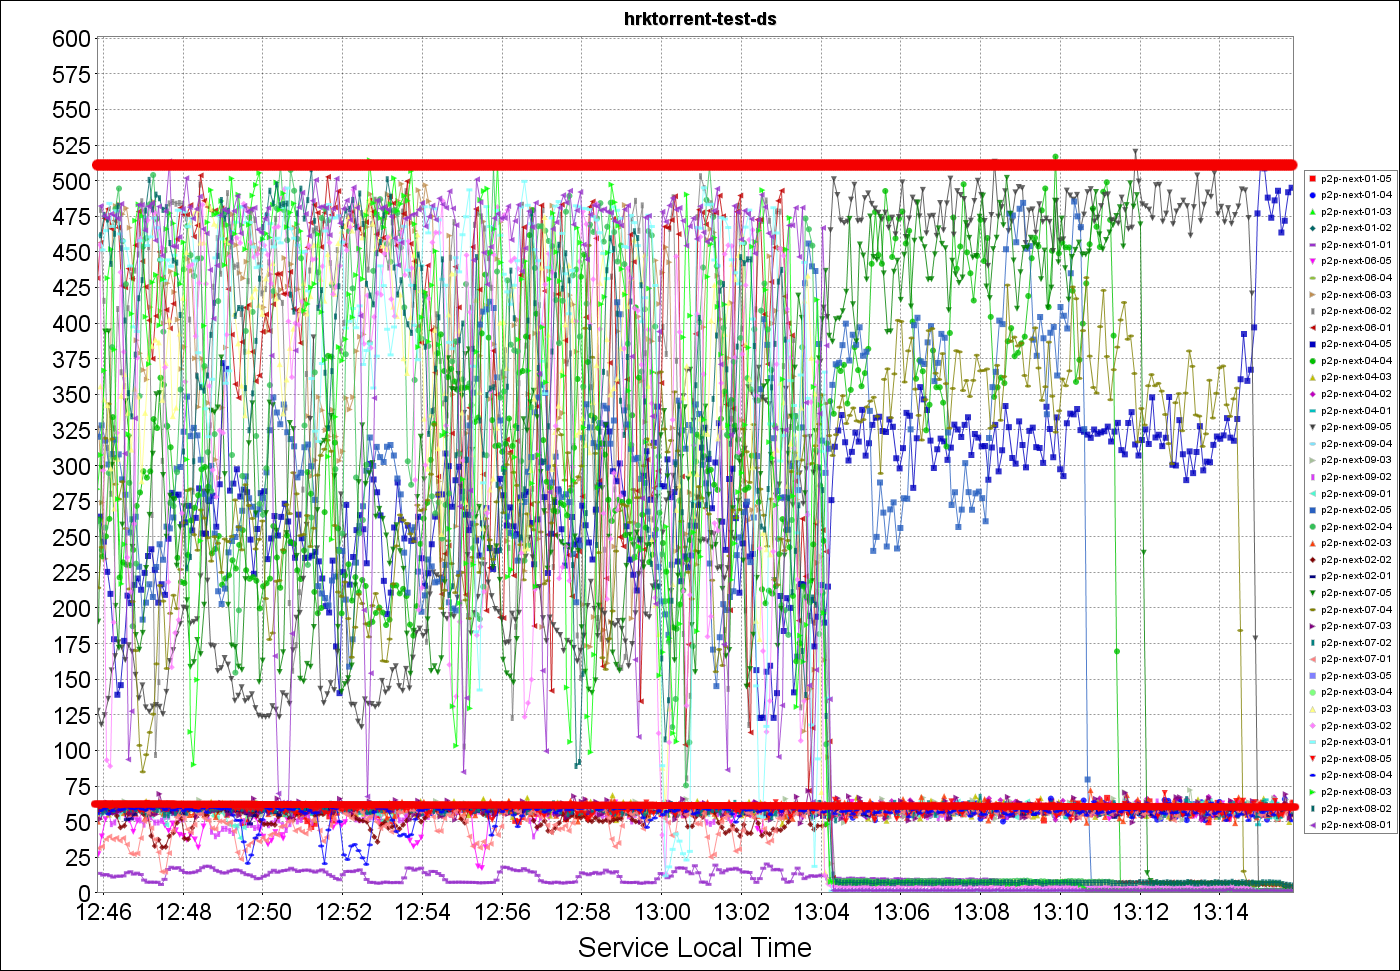
\includegraphics[width=\textwidth]{src/img/virt-infra/test-monalisa-virt-env-stop.png}
    \caption{Download Speed Evolution -- End Phase}
    \label{fig:virt-infra:mon-down-fin}
  \end{minipage}
\end{figure}

Figure~\ref{fig:virt-infra:mon-down-ini} and
Figure~\ref{fig:virt-infra:mon-down-fin} are real time representations of
download speed evolution using MonALISA. The first figure shows the initial
phase (first 10 minutes) of an experiment with the low bandwidth clients
limited by the 64KB/s download speed line, and the high bandwidth clients
running between 100KB/s and 450KB/s. The second figure presents the mid-phase
of an experiment when high bandwidth clients finished downloading. The two
horizontal red lines are the download speed limitations for the two kinds of
clients: 512KB/s for high speed clients and 64KB/s for low speed clients.

Figure~\ref{fig:virt-infra:mon-down-ini} shows the limitation of the low
bandwidth peers while the high bandwidth peers have sparse download speed.
Each high bandwidth client's speed usually follows an up-down evolution, and
an increasing median as time goes by. Low bandwidth clients are limited to
64KB/s while high bandwidth clients fill the range of 64KB/s and 512KB/s. As
time goes the high bandwidth peers tend to stabilize.

Figure~\ref{fig:virt-infra:mon-down-fin} presents the end phase of high
bandwidth peers.  At around 13:05, the high bandwidth clients have completed
their download or are completing it in the following minutes, while the low
bandwidth clients are still downloading. The high bandwidth clients have a
large speed interval, while the low bandwidth clients are ``gathered'' around
the 64KB/s limitation.

\subsection{Performance Evaluation Experiments}

This experimental setup used only six hardware nodes from the infrastructure.
Most of our experiments were simultaneous download sessions. Each system ran a
specific client in the same time and conditions as the other clients. Results
and logging data were collected after each client completed its download.

\subsection{Results}

\begin{figure}
  \centering
  \begin{minipage}{0.8\textwidth}
  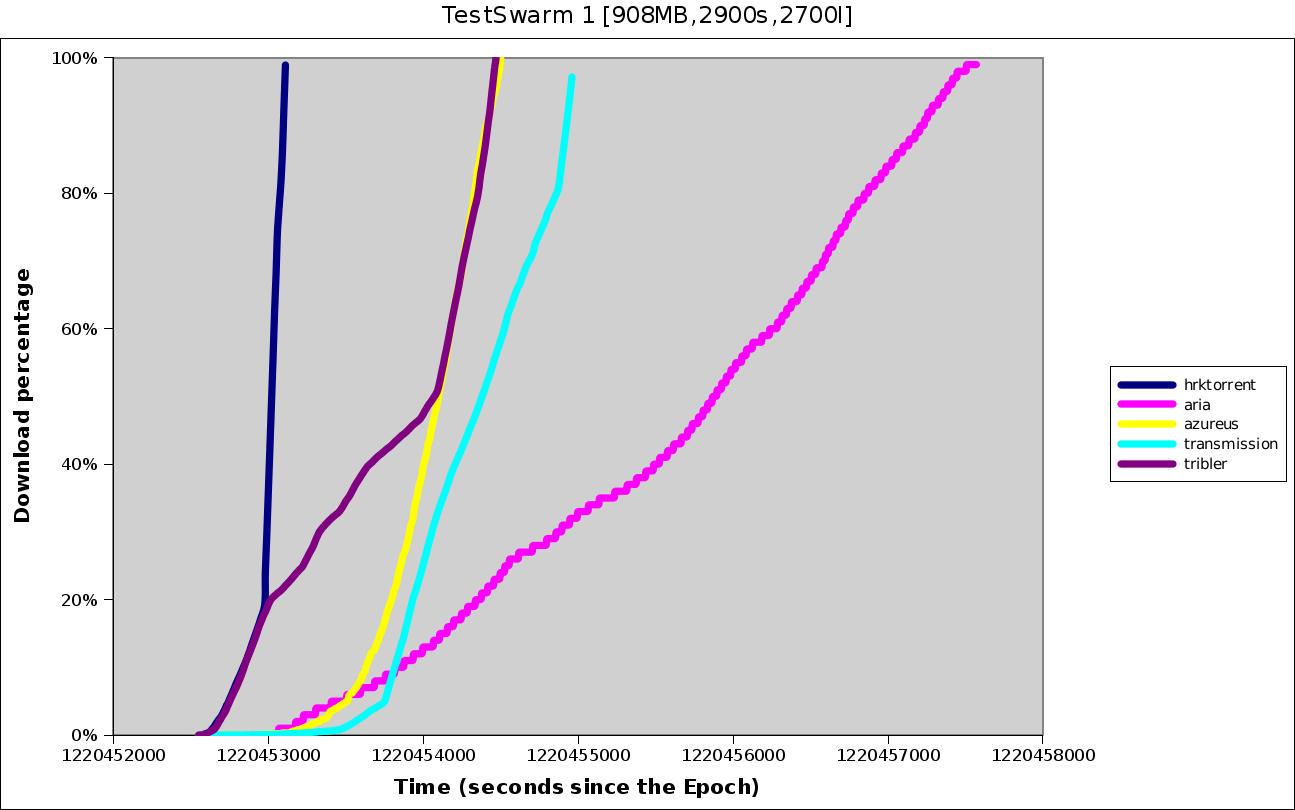
\includegraphics[width=\textwidth]{src/img/virt-infra/test-swarm1-labels}
  \caption{Test Swarm 1}
  \label{fig:virt-infra:ts1}
  \hspace{0.2cm}
  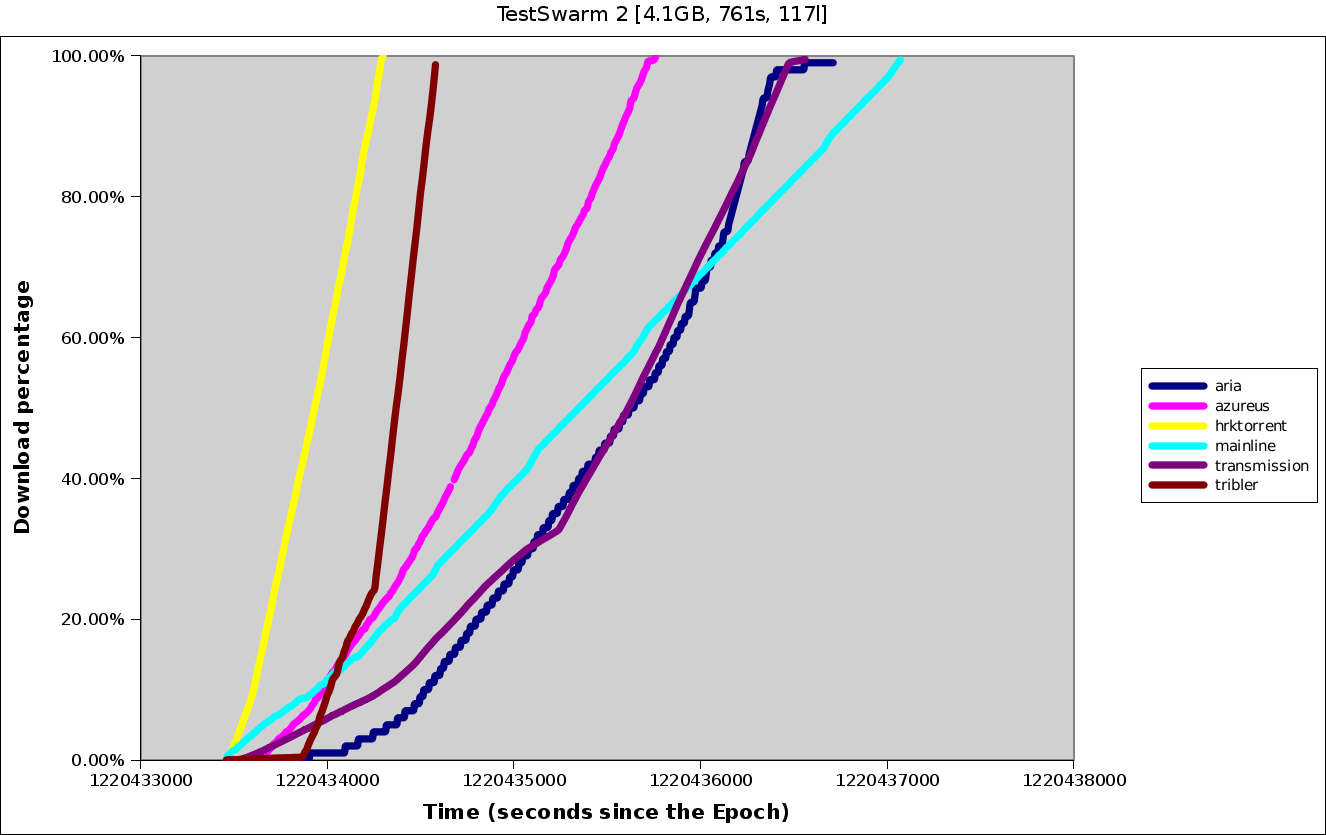
\includegraphics[width=\textwidth]{src/img/virt-infra/test-swarm2-labels}
  \caption{Test Swarm 2}
  \label{fig:virt-infra:ts2}
  \end{minipage}
\end{figure}

Our framework has been used to test different swarms (different .torrent
files). Most scenarios involved simultaneous downloads for all clients. At the
end of each session download status information and extensive logging and
debugging information were gathered from every client.
Figure~\ref{fig:virt-infra:ts1} and Figure~\ref{fig:virt-infra:ts2} are
comparisons between different BitTorrent clients running on the same
environment in the same download scenario.

\begin{table}[ht]
  \centering
  \begin{tabular}{@{}lcccc@{}}
    \toprule
    \textbf{Client} & \textbf{Test1} & \textbf{Test2} & \textbf{Test3} &
    \textbf{Test4} \\
    \midrule
    file size & 908MB & 4.1GB & 1.09GB & 1.09GB	\\
    seeders & 2900 & 761 & 521 & 496	\\
    leechers & 2700 & 117 & 49 & 51	\\
    \midrule
    aria2c & 1h17m & 53m53s & 8m & 10m23s	\\
    azureus & 32m41s & 38m33s & N/A & 7m	\\
    bittorrent & 4h53m & 60m39s & 26m & 14m	\\
    libtorrent & \textbf{9m41s} & \textbf{15m13s} & \textbf{2m30s} & \textbf{2m14s}	\\
    transmission & 40m46s & 53m & 7m & 5m	\\
    tribler & 34m & 21m & N/A & N/A		\\
    \bottomrule
  \end{tabular}
  \caption{Test Swarms Results}
  \label{table:virt-infra:testsw}
\end{table}

Table~\ref{table:virt-infra:testsw} presents a comparison of the BitTorrent
clients in four different scenarios. Each scenario means a different swarm.
Although many data were collected, only the total download time is featured in
the table.

The conclusions drawn after result analysis were:

\begin{itemize}
  \item hrk/libttorrent is continuously surpassing the other clients in 
  different scenarios;
  \item tribler, azureus and transmission are quite good clients but lag 
  behind hrktorrent;
  \item mainline and aria are very slow clients and should be dropped from 
  further tests;
  \item swarms that are using sharing ratio enforcement offer better 
  performance; a file is downloaded at least 4 times faster within a swarm 
  using sharing ratio enforcement.
\end{itemize}

\subsection{Deploying the Rendering Engine}

A class of specific experiments made use of 40 virtualized peers which were
configured to use bandwidth limitations. Half of the peers (20) were
considered to be high-bandwidth peers, while the other half were considered to
be low-bandwidth peers. The high-bandwidth peers were limited to 512KB/s
download speed and 256KB/s upload speed and the low-bandwidth peers were
limited to 64KB/s download speed and 32KB/s upload speed.

\begin{figure}[h]
  \centering
  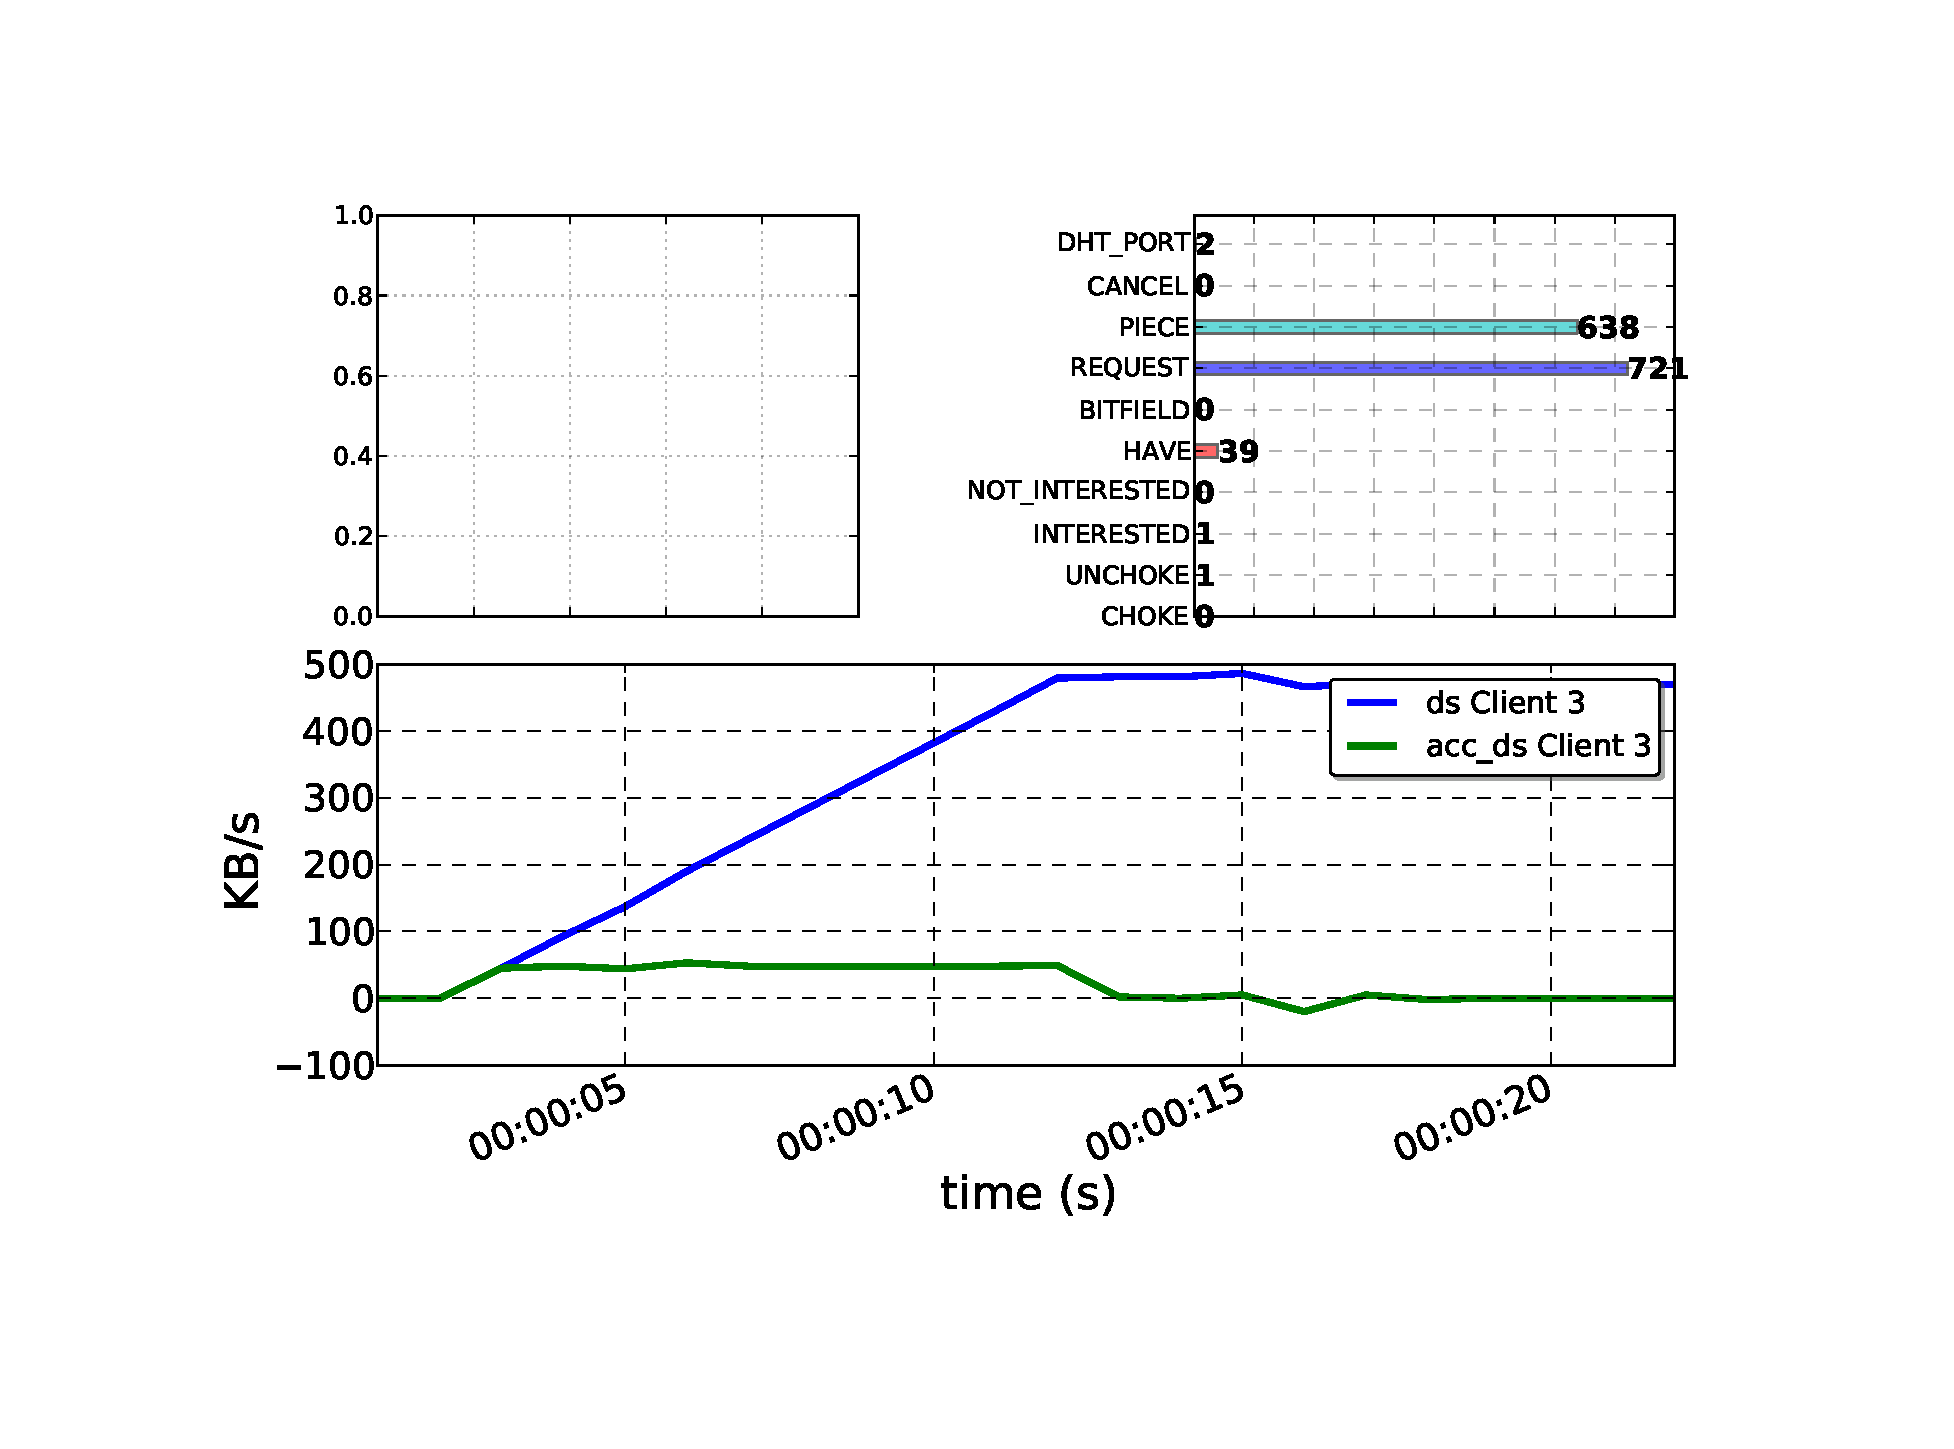
\includegraphics[trim = 3.8cm 4cm 4.3cm 10.7cm, clip, width =
0.7\textwidth]{src/img/virt-infra/test3}
  \caption{Download speed/acceleration evolution (libtorrent BitTorrent client)}
  \label{fig:virt-infra:down-acc}
\end{figure}

\begin{figure}[h]
  \centering
    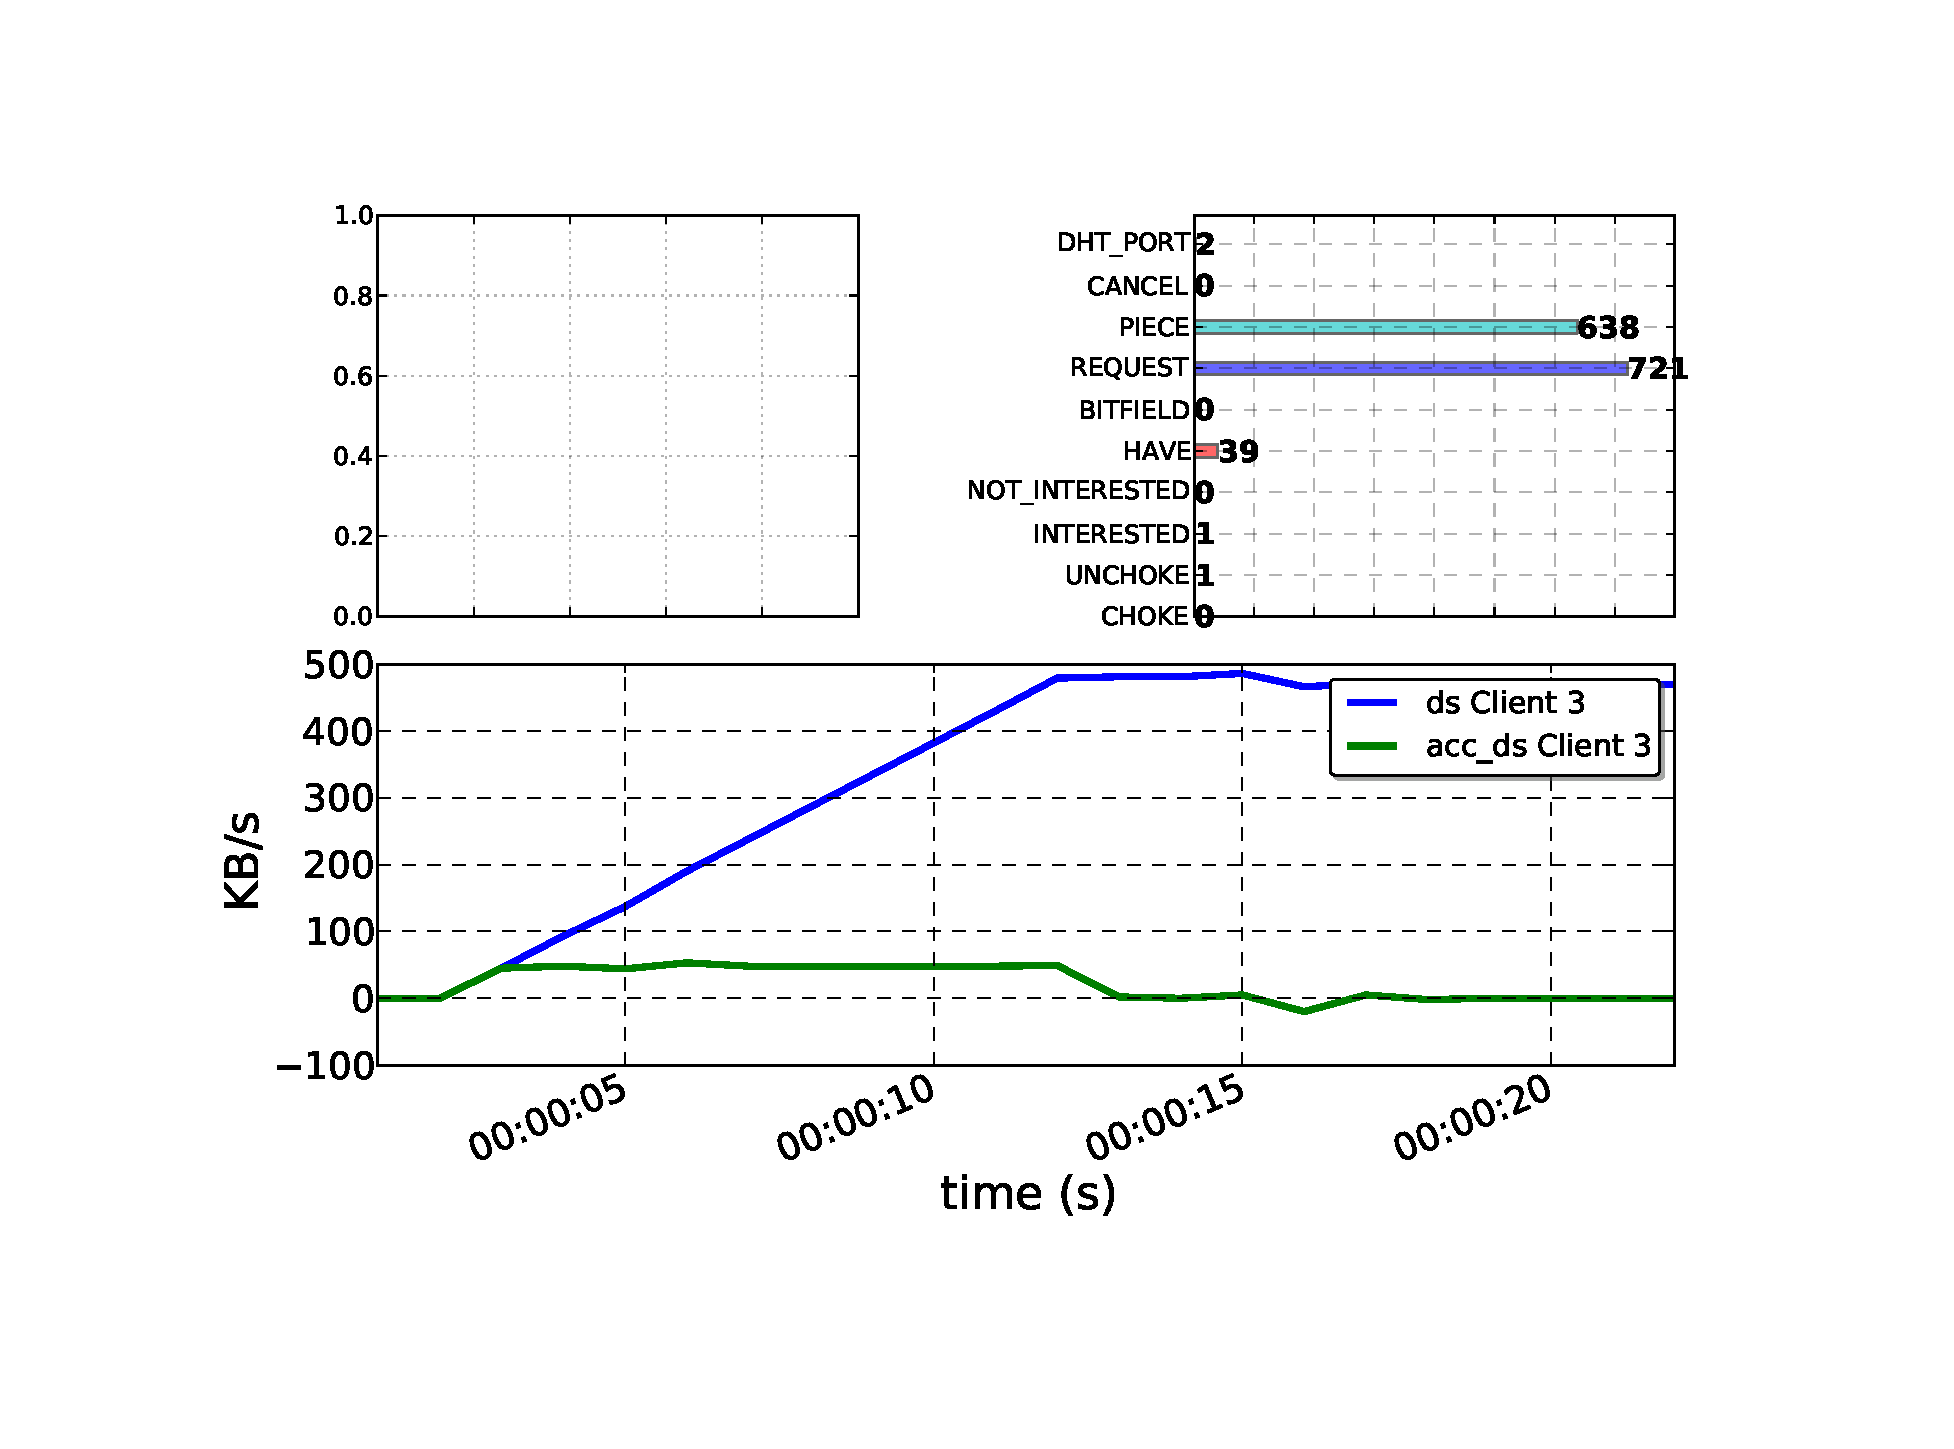
\includegraphics[trim = 15.9cm 13.5cm 4.3cm 3cm, clip, width =
0.7\textwidth]{src/img/virt-infra/test3}
  \caption{BitTorrent protocol messages (20 seconds)}
  \label{fig:virt-infra:proto-msg}
\end{figure}

Figure~\ref{fig:virt-infra:down-acc} displays a 20 seconds time-based
evolution of the download speed and acceleration of a peer running the
libtorrent client.  Acceleration is high during the first 12 seconds, when a
peer reaches its maximum download speed of around 512KB/s. Afterwards, the
peer's download speed is stabilized and its acceleration is close to 0.

All non-seeder peers display a similar start-up pattern. There is an initial
10-12 seconds bootstrap phase with high acceleration and rapid reach of its
download limit, and a stable phase with the acceleration close to 0.

Figure~\ref{fig:virt-infra:proto-msg} displays messages exchanged during the
first 20 seconds of a peer's download session, in direct connection with
Figure~\ref{fig:virt-infra:down-acc}. The peer is quite aggressive in its
bootstrap phase and manages to request and receive a high number of pieces.
Almost all requests sent were replied with a block of data from a piece of the
file.

The download speed/acceleration time-based evolution graph and the protocol
messages numbering are usually correlated and allow detailed analysis of a
peer's behaviour. Our goal is to use this information to discover weak spots
and areas to be improved in a given implementation or swarm or network
topology.

\section{Conclusion}
\label{sec:virt-infra:conclusion}

In order to create an extensible, realistic and automated environment for
deploying Peer-to-Peer trials, we have constructed a virtualized
infrastructure. The infrastructure provides the means for creating
Peer-to-Peer nodes and designing the network connection between them to an
as-close-to reality as possible topology. Through the use of virtualization,
we were able to reliably and efficiently use less than a dozen of commodity
hardware systems to simulate a complete set of more than a hundred peers.

OpenVZ was choosen as the virtualization solution. A lightweight operating
system-level virtualization solution, OpenVZ provided the light overhead and
easy deployment and interaction required, though problems were encountered
when applying bandwidth limitation options. OpenVZ provides a low memory
footprint and low overhead albeit at the price of less separation between
various processes. Due to its low memory footprint it was fairly easy to
deploy tens of virtual nodes on top of a modest commodity hardware system.

A variety of tools have been employed to allow a realistic behavior and ensure
automation. SSH has been used as the protocol for directly interacting with
nodes and sending commands for building up the infrastructure or interacting
with clients. iptables and tc have been employed for networking features such
as firewalls and bandwidth limitations. Shell scripting has been used for
automating various components of the infrastructure.

A diversity of BitTorrent clients have been used as basis of comparison and
have been integrated through scripting in the infrastructure. Some of these
clients have been instrumented for easy automation and providing required
information. Ranging from Tribler to Vuze, clients are configured to run
within a given OpenVZ container and be part of the simulated swarm.

Connection dropouts have been simulated through various means such as stopping
the client, suspending it or disabling the interface. Connection dropout
simulation has been integrated in the virtualized infrastructure in order to
ensure churning in a Peer-to-Peer swarm. Result have signaled a similarity of
the methods and supported the use of suspending the client due to its easy
integration in the swarm management framework.

Experiments and trials make use of the infrastructure such that it is able to
simulate a swarm consisting of more than 100 clients. We differentiate between
an internal swarm -- consisting solely of simulated virtualized nodes, and
external swarm -- combining simulated virtualized nodes with real nodes from
the Internet. A specific type of experiments have been directing at providing
a performance overview and comparison between various clients.
